% !TeX root = PM_01.tex
%% 
%% Copyright 2019-2024 Elsevier Ltd
%% 
%% Version 2.4
%% 
%% This file is part of the 'CAS Bundle'.
%% --------------------------------------
%% 
%% It may be distributed under the conditions of the LaTeX Project Public
%% License, either version 1.2 of this license or (at your option) any
%% later version.  The latest version of this license is in
%%    http://www.latex-project.org/lppl.txt
%% and version 1.2 or later is part of all distributions of LaTeX
%% version 1999/12/01 or later.
%% 
%% The list of all files belonging to the 'CAS Bundle' is
%% given in the file `manifest.txt'.
%% 
%% Template article for cas-dc documentclass for 
%% double column output.

%\documentclass[a4paper,fleqn,longmktitle]{cas-dc}
\documentclass[a4paper,fleqn]{cas-dc}

%\usepackage[authoryear,longnamesfirst]{natbib}
%\usepackage[authoryear]{natbib}
\usepackage[numbers]{natbib}

% ------------------------------------------------------------
% Figures and TikZ
% ------------------------------------------------------------
\usepackage{graphicx}
\graphicspath{{figs/}}
\usepackage{placeins}
\usepackage{tikz}
\usetikzlibrary{arrows.meta,positioning,shapes.geometric}

% Keep figures near their source locations; do not load endfloat.
% ------------------------------------------------------------
% Equation spacing
% ------------------------------------------------------------
\setlength{\abovedisplayskip}{6pt}
\setlength{\belowdisplayskip}{6pt}
\setlength{\abovedisplayshortskip}{4pt}
\setlength{\belowdisplayshortskip}{4pt}
\setlength{\textfloatsep}{3.5pt}
\setlength{\intextsep}{3.5pt}



% ------------------------------------------------------------
% Figure-caption font
% Make captions match the main document font and size
% ------------------------------------------------------------
\usepackage{etoolbox}

\ExplSyntaxOn

\patchcmd{\__make_fig_caption:nn}
{\sffamily\small}
{\normalfont\normalsize}
{}{}

\patchcmd{\__make_fig_caption:nn}
{\sffamily\small}
{\normalfont\normalsize}
{}{}

\patchcmd{\__make_fig_caption:nn}
{\sffamily\small}
{\normalfont\normalsize}
{}{}

\ExplSyntaxOff
% ------------------------------------------------------------
% Figure caption formatting for Elsevier cas-dc
% ------------------------------------------------------------
\ExplSyntaxOn

\cs_set:Npn \__make_fig_caption:nn #1#2
{
	\l_fig_align_tl
	\skip_vertical:N \l_fig_abovecap_skip
	
	\setbox\cascaptionbox=\hbox{
		\normalfont\normalsize
		#1:~#2
	}
	
	\ifdim\the\wd\cascaptionbox<\dim_use:N\l_fig_width_dim\relax
	\parbox{\l_fig_width_dim}{
		\unskip\ignorespaces
		\hfil
		\normalfont\normalsize
		#1:~#2
		\hfil\par
	}
	\else
	\parbox{\l_fig_width_dim}{
		\rightskip=0pt
		\unskip\ignorespaces
		\normalfont\normalsize
		#1:~#2
		\par
	}
	\fi
	
	\skip_vertical:N \l_fig_belowcap_skip
}

\ExplSyntaxOff

%%%Author definitions
\def\tsc#1{\csdef{#1}{\textsc{\lowercase{#1}}\xspace}}
\tsc{WGM}
\tsc{QE}
\tsc{EP}
\tsc{PMS}
\tsc{BEC}
\tsc{DE}
%%%

\begin{document}
	\let\WriteBookmarks\relax
	\def\floatpagepagefraction{1}
	\def\textpagefraction{.001}
	\shorttitle{Leveraging social media news}
	\shortauthors{K Umamahesh et~al.}
	
	\title [mode = title]{This is a specimen $a_b$ title}                      
	\tnotemark[1,2]
	
	
	
	\author[1]{Kushal Umamahesh}
	\ead{k.kushalumamahesh.959@cranfield.ac.uk}
	
	\author[1]{Tamás Józsa}
	
	\affiliation[1]{
		organization={Centre for Assured and Connected Autonomy, Faculty of Engineering and Applied Sciences, Cranfield University},
		city={Cranfield},
		postcode={MK43 0AL},
		state={Bedfordshire},
		country={United Kingdom}
	}
	
	
	
	
	\fnmark[2]
	\ead{wjh@example.org}
	\ead[URL]{https://www.university.org}
	
	\credit{Data curation, Writing - Original draft preparation}
	
	
	
	\cortext[cor1]{Corresponding author}
	\cortext[cor2]{Principal corresponding author}
	
	
	
	\begin{abstract}
		Porous airfoils offer a passive means of modifying aerodynamic loading through pressure-driven flow within internal pathways. This study develops a coupled aerodynamic–hydraulic framework for a NACA 0018 airfoil, combining a source–vortex panel method with rectangular-channel flow models. Three configurations are investigated: chordwise horizontal channels, vertical channels connecting the pressure and suction surfaces, and a combined horizontal–vertical arrangement. The results show that aerodynamic performance depends strongly on pore orientation and connectivity. Horizontal channels  redistribute pressure between chordwise locations on the same surface and increase lift at positive angles of attack, with stronger effects at larger pore heights. Vertical pore promote pressure equalisation between the pressure and suction surfaces and reduce lift relative to the impermeable airfoil. In the combined configuration, these mechanisms interact through the external flow field, giving a response closer to that of the solid airfoil. Pressure and velocity difference fields show that the strongest flow modifications occur near the pore openings. These results demonstrate that porous-airfoil performance is governed not simply by porosity, but by the orientation, location and hydraulic connectivity of the internal channels. 
	\end{abstract}
	
	\begin{graphicalabstract}
		
	\end{graphicalabstract}
	
	\begin{highlights}
		\item Research highlights item 1
		\item Research highlights item 2
		\item Research highlights item 3
	\end{highlights}
	
	\begin{keywords}
		Porous airfoil \sep Passive flow control \sep Panel method \sep Pressure-driven internal flow \sep Anisotropic porosity \sep 
	\end{keywords}
	
	
	\maketitle
	
	\section{Introduction}
	\label{sec:introduction}
	
	Improving airfoil performance without relying on powered control systems remains an important objective in aerospace and energy applications. Conventional high-lift and flow-control devices can be effective, but they may introduce mechanical complexity, additional mass, maintenance requirements, and changes that disrupt the smooth external surface of the airfoil. Passive flow-control concepts provide an alternative strategy in which the pressure field surrounding an aerodynamic body supplies the energy required to modify the flow. Porous surfaces, permeable regions, localised pores, and internal channels employ this principle by permitting fluid transport between regions of unequal pressure. Their effectiveness, however, depends on the placement of the pores, the manner in which they are connected, and the strength of the interaction between the resulting surface normal flow and the external aerodynamic field.
	
	
	Early investigations established that surface porosity can substantially modify the pressure distribution and aerodynamic forces acting on an airfoil, while also demonstrating that porosity is not inherently beneficial. Mineck and Hartwich examined full-chord porosity on a NACA~0012 airfoil under transonic-flow conditions and found that the porous surface generally reduced the rate at which lift increased with angle of attack and increased drag for a given normal-force coefficient \cite{Mineck1996FullChordPorosity}. Experiments by Aldheeb et al. similarly showed that increasing porosity reduced the rate of lift increase. They also found that a small amount of porosity initially reduced drag, whereas further increases in porosity caused drag to rise \cite{Aldheeb2018PorousAirfoilsWings}. Together, these findings show that allowing pressure to equalise freely across the airfoil can reduce the pressure difference required for lift generation and may adversely affect aerodynamic performance. Effective passive flow control therefore requires selective permeability or controlled connectivity rather than indiscriminate porosity across the airfoil.
	
	
	Reduced-order models have provided important insight into how distributed permeability affects airfoil aerodynamics. Hajian and Jaworski introduced a steady thin-airfoil formulation in which a local Darcy condition relates the pressure difference across the airfoil to the flow through a chordwise distribution of porosity \cite{Hajian2017PorosityGradients}. Luesutthiviboon et al. assessed a related thin-airfoil model for partially porous airfoils and found that its accuracy decreased when the porous region was small or the flow resistance was low \cite{Luesutthiviboon2019ThinAirfoilAssessment}. Baddoo et al. subsequently extended porous-airfoil modelling to unsteady motion and gust response by including the effects of flow resistance and the inertia of the fluid moving through the porous surface \cite{Baddoo2021UnsteadyPorousAerofoils}. These models are computationally efficient and explain the relationship between pressure difference, flow resistance, and the resulting aerodynamic forces. However, thin-airfoil formulations do not represent the finite thickness of an airfoil. Their porous boundary conditions also primarily describe local flow between the pressure and suction surfaces through distributed or homogenised porous material, rather than flow through finite-length internal channel connecting selected and spatially separated surface pores.
	
	
	Experiments and high-fidelity simulations also show that the internal structure and directionality of the permeable region are important. Hanna and Spedding studied a NACA~0012 wing containing discrete wall-normal holes and observed that a small degree of porosity modified the lift response around zero incidence while maintaining comparable lift-to-drag performance within the experimental uncertainty over much of the tested range \cite{Hanna2019PorosityModerateRe}. For a NACA~0018 airfoil, Zhu et al. compared fully porous and suction-side porous trailing-edge arrangements and found distinct aerodynamic and acoustic responses, demonstrating the sensitivity of the outcome to porous placement and cross-surface pressure release \cite{Zhu2023NACA0018PorousTrailingEdge}. Li et al. compared an isotropic porous medium with directionally constrained straight holes using large-eddy simulation and showed that aerodynamic behaviour depends not only on porous extent and porosity but also on the internal flow direction permitted by the structure \cite{Li2023PartiallyPorousAirfoils}. Taken together, these studies show that a bulk porosity or permeability value alone is insufficient to describe the aerodynamic function of a designed internal architecture.
	
	An alternative class of passive devices uses internal slots or channels to transport fluid from a region of high pressure to one of lower pressure. Acarer optimised passive slots for the DU12W262 airfoil and reported an improvement in the peak lift-to-drag ratio, demonstrating the potential of pressure-driven flow through internal channels to improve aerodynamic performance \cite{Acarer2020DU12W262PassiveFlow}. Kestel et al. used passive flow through internal channels to modify the separated vortex structure over a non-slender delta wing, directly demonstrating fluid transport driven by the natural pressure difference between connected surfaces \cite{Kestel2020PassiveBleeding}. More recently, Bahadi et al. conducted a parametric investigation of a curved internal slot in a NACA~4412 airfoil and reported increased aerodynamic performance at high angles of attack for selected inlet, taper, and curvature configurations \cite{Bahadi2026CurvedPassiveSlot}. These studies demonstrate that internal pressure-driven connections have been investigated previously. Therefore, the contribution of the present study is not the initial introduction of passive connectivity, but the development of a general reduced-order framework for modelling multiple pairs of pores connected by independent internal channels. Previous investigations have generally focused on a specific slot geometry using experiments or Reynolds-averaged Navier--Stokes calculations.
	
	
	Porous-airfoil design is increasingly being treated as an optimisation problem because aerodynamic performance depends on several interacting geometric and material variables. Zamani et al. applied a parameter-screening and optimisation procedure to a porous NACA~0015 airfoil for static-stall control, varying the dimensions and location of the porous region, together with its porosity and cell size \cite{Zamani2026NACA0015PorousStall}. This work demonstrates the value of systematic design exploration, although the porous layer is represented using distributed material properties. For airfoils with individual internal channels, the design variables include which surface pores are connected, where the pores are positioned, the length, orientation, and height of each channel, and whether the channels connect pores on the same surface or link the pressure and suction surfaces. Exploring this larger range of possible channel arrangements exclusively through viscous computational fluid dynamics or experiments would be computationally expensive during the preliminary design stage.
	
	
	Panel methods bridge the gap between simplified analytical thin-airfoil models and computationally expensive viscous-flow simulations. The foundational work of Hess and Smith established a boundary-element representation of potential flow by distributing singularities along the boundary of the geometry. This approach enables the pressure field around a geometrically resolved body to be calculated without discretising the surrounding fluid domain \cite{HessSmith1967PotentialFlow}. The subsequent review by Hess documented the development, capabilities, and limitations of panel methods as efficient aerodynamic boundary-integral techniques \cite{Hess1990PanelMethods}, while Birk provided a modern, implementation-focused description of the Hess--Smith method using constant-strength source and doublet distributions \cite{Birk2022HessSmithGuide}. For a two-dimensional lifting airfoil, a source distribution enforces the surface-normal boundary condition, while circulation and a trailing-edge Kutta condition produce the lifting solution. This structure is particularly suitable for the present problem because the standard impermeability condition can be modified locally by prescribing a normal flow velocity at each surface pore. The calculated surface velocity determines the pressure coefficient, from which the pressure difference between each pair of connected pores is obtained to drive the internal channel flow. Panel methods are also computationally inexpensive, allowing repeated calculations for numerous channel arrangements, pore sizes, and angles of attack.
	
	
	Established viscous--inviscid methods show how potential-flow panel calculations can be combined with boundary-layer models to provide a more complete analysis of airfoil performance. Drela and Giles developed a strongly coupled viscous--inviscid method for transonic and low-Reynolds-number airfoils by combining an inviscid outer-flow solution with integral boundary-layer equations \cite{DrelaGiles1987ViscousInviscid}. XFOIL later implemented a similar approach in a computationally efficient airfoil-analysis and design tool, using a linear-vorticity panel method for the inviscid flow together with integral boundary-layer equations and a transition-prediction model \cite{Drela1989XFOIL}. Although these methods predict viscous effects that are not included in the present formulation, their use of panel methods for the external flow supports the efficient calculation of surface-pressure distributions using potential-flow theory. In the present study, XFOIL is used only as a reference for the solid-airfoil baseline. The proposed external-flow solver remains inviscid so that the pressure-driven aero--hydraulic interaction can be isolated and evaluated at a low computational cost. This modelling choice also makes the method suitable for preliminary design screening, after which selected channel configurations can be investigated using viscous computational fluid dynamics or experiments.
	
	
	The reviewed literature therefore covers distributed Darcy-type surfaces, homogenised porous media, pores oriented normal to the airfoil surface, individual passive slots, and established potential-flow panel formulations. However, a modelling gap remains between local permeability boundary conditions and high-fidelity simulations of specific internal geometries. In particular, limited attention has been given to a panel-based reduced-order framework that explicitly connects selected pairs of surface pores using finite-length internal channels, calculates the pressure-driven flow through each channel, and uses the resulting inflow and outflow velocities at the pores to update the external aerodynamic solution. The systematic comparison of channels connecting spatially separated pores on the same surface, channels connecting the pressure and suction surfaces, and a combined arrangement containing both channel types as hydraulically independent connections also remains underexplored. Addressing this gap would provide a computationally efficient method for screening many candidate channel layouts before conducting higher-fidelity viscous simulations and experimental validation.
	
	
	Accordingly, the present study develops a two-dimensional coupled aero--hydraulic framework for a NACA~0018 airfoil. The external flow is represented by a steady, incompressible, inviscid, and irrotational source--vortex panel method with a Kutta condition. Selected pairs of surface pores are connected by passive rectangular channels, and the pressure difference between the paired pores determines the internal flow according to a hydraulic-resistance relation. The resulting surface-normal flow velocities at the pores are iteratively coupled with the external panel solution. Three channel arrangements are examined: four chordwise channels connecting pores on the same surface, four vertical channels connecting the pressure and suction surfaces, and a combined arrangement containing all eight channels as hydraulically independent connections. Channel heights of 8, 9, and 10~mm are assessed over angles of attack from $-5^{\circ}$ to $15^{\circ}$ at a chord Reynolds number of $5\times10^{5}$. The results are compared with those of the solid airfoil and an XFOIL reference solution.
	
	
	The main contribution of this study is a reduced-order representation of finite-length internal channels connecting selected pairs of surface pores within a coupled external-flow and internal-channel model. The formulation allows different channel arrangements to be evaluated using a consistent aerodynamic model and demonstrates the relationships among the pressure difference between connected pores, internal flow rate, surface-normal flow velocity, pressure distribution, lift, pitching moment, and pressure-based streamwise force. The method is intended for rapid preliminary assessment and comparison of candidate channel layouts. Because the external-flow model does not resolve boundary layers, skin-friction drag, flow separation, or stall, the results are interpreted as inviscid aerodynamic trends and used to select promising configurations for subsequent viscous computational analysis and experimental validation.
	
	
	
	
	% ============================================================
	% NUMERICAL METHODOLOGY — manuscript section
	% ============================================================
	% Required packages: amsmath, graphicx, tikz.
	% TikZ libraries: positioning, arrows.meta, shapes.geometric.
	% Load both the introduction and methods bibliography files from the MAIN file.
	% AUTHOR CHECK: the table retains the manuscript study values. The latest
	% config(3).py instead defaults to Re_c=1e6, sweep H=6/7/8 mm and single H=17 mm.
	% Confirm which settings generated the reported results before submission.
	\section{Methods}
	\label{sec:numerical_methodology}
	
	\subsection{Modelling framework and assumptions}
	\label{subsec:overall_framework}
	
	A two-dimensional coupled aero--hydraulic model was developed for a
	NACA~0018 airfoil containing passive internal channels. In this study, a
	\emph{pore} denotes the finite surface region at which a channel intersects
	the airfoil boundary, whereas a \emph{channel} denotes the finite-length
	internal connection between two pores. The external flow is represented by a
	steady source--vortex panel method, and the flow in each channel is represented
	by a one-dimensional pressure-loss model per unit span. The two models exchange
	surface pressure and pore-normal velocity until their flow rates are mutually
	consistent.
	
	The external model assumes incompressible, inviscid and irrotational flow. It
	therefore does not resolve boundary layers, skin friction, separation, transition
	or stall. The internal model assumes a straight, smooth, constant-height
	rectangular channel described by its cross-sectionally averaged velocity. Entrance turning,
	three-dimensional pore-mouth flow and jet mixing are not resolved explicitly; their
	treatment in the reduced energy closure is stated in
	Section~\ref{subsec:internal_channel_model}. Accordingly, the method is intended
	for rapid comparison and screening of channel layouts rather than as a substitute
	for viscous computational-fluid-dynamics or experimental analysis.
	
	The first flow estimate is calculated from the solid-airfoil pressure
	distribution, with zero surface-normal velocity. The pressure at each pore
	is supplied to the channel model to obtain an initial channel flow rate.
	These flows produce suction and blowing at the pores, which change the external
	pressures. The channel flow rates are therefore adjusted until they agree with
	the flow rates driven by the updated pressures. A nearby converged solution
	is used as the initial estimate for subsequent cases where available.
	Figure~\ref{fig:coupled_solution_workflow} summarises the calculation.
	
	\begin{figure}[pos=!htbp]
		\centering
		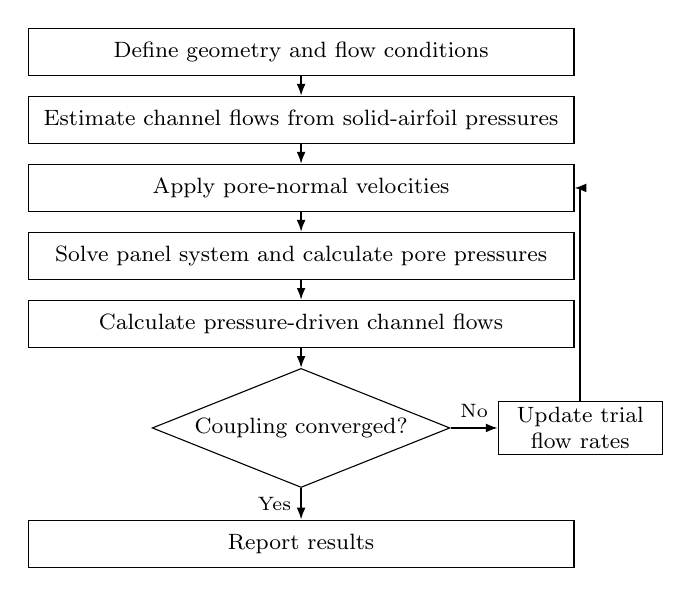
\begin{tikzpicture}[
			font=\normalfont\footnotesize,
			node distance=2.5mm,
			process/.style={
				rectangle,draw,align=center,
				text width=0.56\linewidth,
				minimum height=6mm,
				inner sep=2pt
			},
			decision/.style={
				diamond,draw,aspect=2.5,align=center,
				text width=0.24\linewidth,
				inner sep=1pt
			},
			arrow/.style={-{Latex[length=1.5mm]},semithick}
			]
			
			\node[process] (geometry)
			{Define geometry and flow conditions};
			
			\node[process,below=of geometry] (guess)
			{Estimate channel flows from solid-airfoil pressures};
			
			\node[process,below=of guess] (map)
			{Apply pore-normal velocities};
			
			\node[process,below=of map] (panel)
			{Solve panel system and calculate pore pressures};
			
			\node[process,below=of panel] (hydraulic)
			{Calculate pressure-driven channel flows};
			
			\node[decision,below=of hydraulic] (converged)
			{Coupling converged?};
			
			\node[process,below=4mm of converged] (report)
			{Report results};
			
			\node[
			process,
			right=6mm of converged,
			text width=0.16\linewidth
			] (retry) {Update trial flow rates};
			
			\draw[arrow] (geometry) -- (guess);
			\draw[arrow] (guess) -- (map);
			\draw[arrow] (map) -- (panel);
			\draw[arrow] (panel) -- (hydraulic);
			\draw[arrow] (hydraulic) -- (converged);
			
			\draw[arrow] (converged) --
			node[left,font=\scriptsize]{Yes} (report);
			
			\draw[arrow] (converged) --
			node[above,font=\scriptsize]{No} (retry);
			
			\draw[arrow] (retry.north) |- (map.east);
			
		\end{tikzpicture}
		
		\caption{Coupled aero--hydraulic solution procedure.}
		\label{fig:coupled_solution_workflow}
	\end{figure}
	
	\subsection{Airfoil and channel geometry}
	\label{subsec:airfoil_channel_geometry}
	
	The closed NACA four-digit profile is generated from the standard analytical
	ordinates \cite{Ladson1996NACAAirfoils}. The coefficient $-0.1036$ is used for
	the fourth-order thickness term to obtain a closed trailing edge. Cosine-spaced
	points are placed on each surface and joined by $N$ straight panels. Panel $i$
	has length $S_i$, control point $(x_i,y_i)$, unit tangent
	$\boldsymbol t_i=(t_{x,i},t_{y,i})$ and outward unit normal
	$\boldsymbol n_i=(n_{x,i},n_{y,i})$.
	
	Three layouts are considered:
	\begin{enumerate}
		\item \textbf{Chordwise layout:} four independent same-surface channels,
		comprising two on the upper surface and two on the lower surface;
		\item \textbf{Cross-surface layout:} four independent channels connecting
		the lower and upper surfaces at chordwise positions distributed from
		approximately $x/c=0.10$ to $0.89$; and
		\item \textbf{Combined layout:} all eight channels from the preceding
		layouts, retained as hydraulically independent connections with no internal
		junction or exchange of flow between channels.
	\end{enumerate}
	The layouts are shown in Figure~\ref{fig:porous_models}. A crossing of projected
	channel centrelines in the two-dimensional drawing does not create a hydraulic
	connection. Such crossings represent an idealised independent-channel model,
	not a resolved, physically intersecting two-dimensional channel geometry; a
	realisation would require separation of the channels. Surface pores are not
	permitted to overlap.
	
	\begin{figure}[pos=!htbp]
		\centering
		
		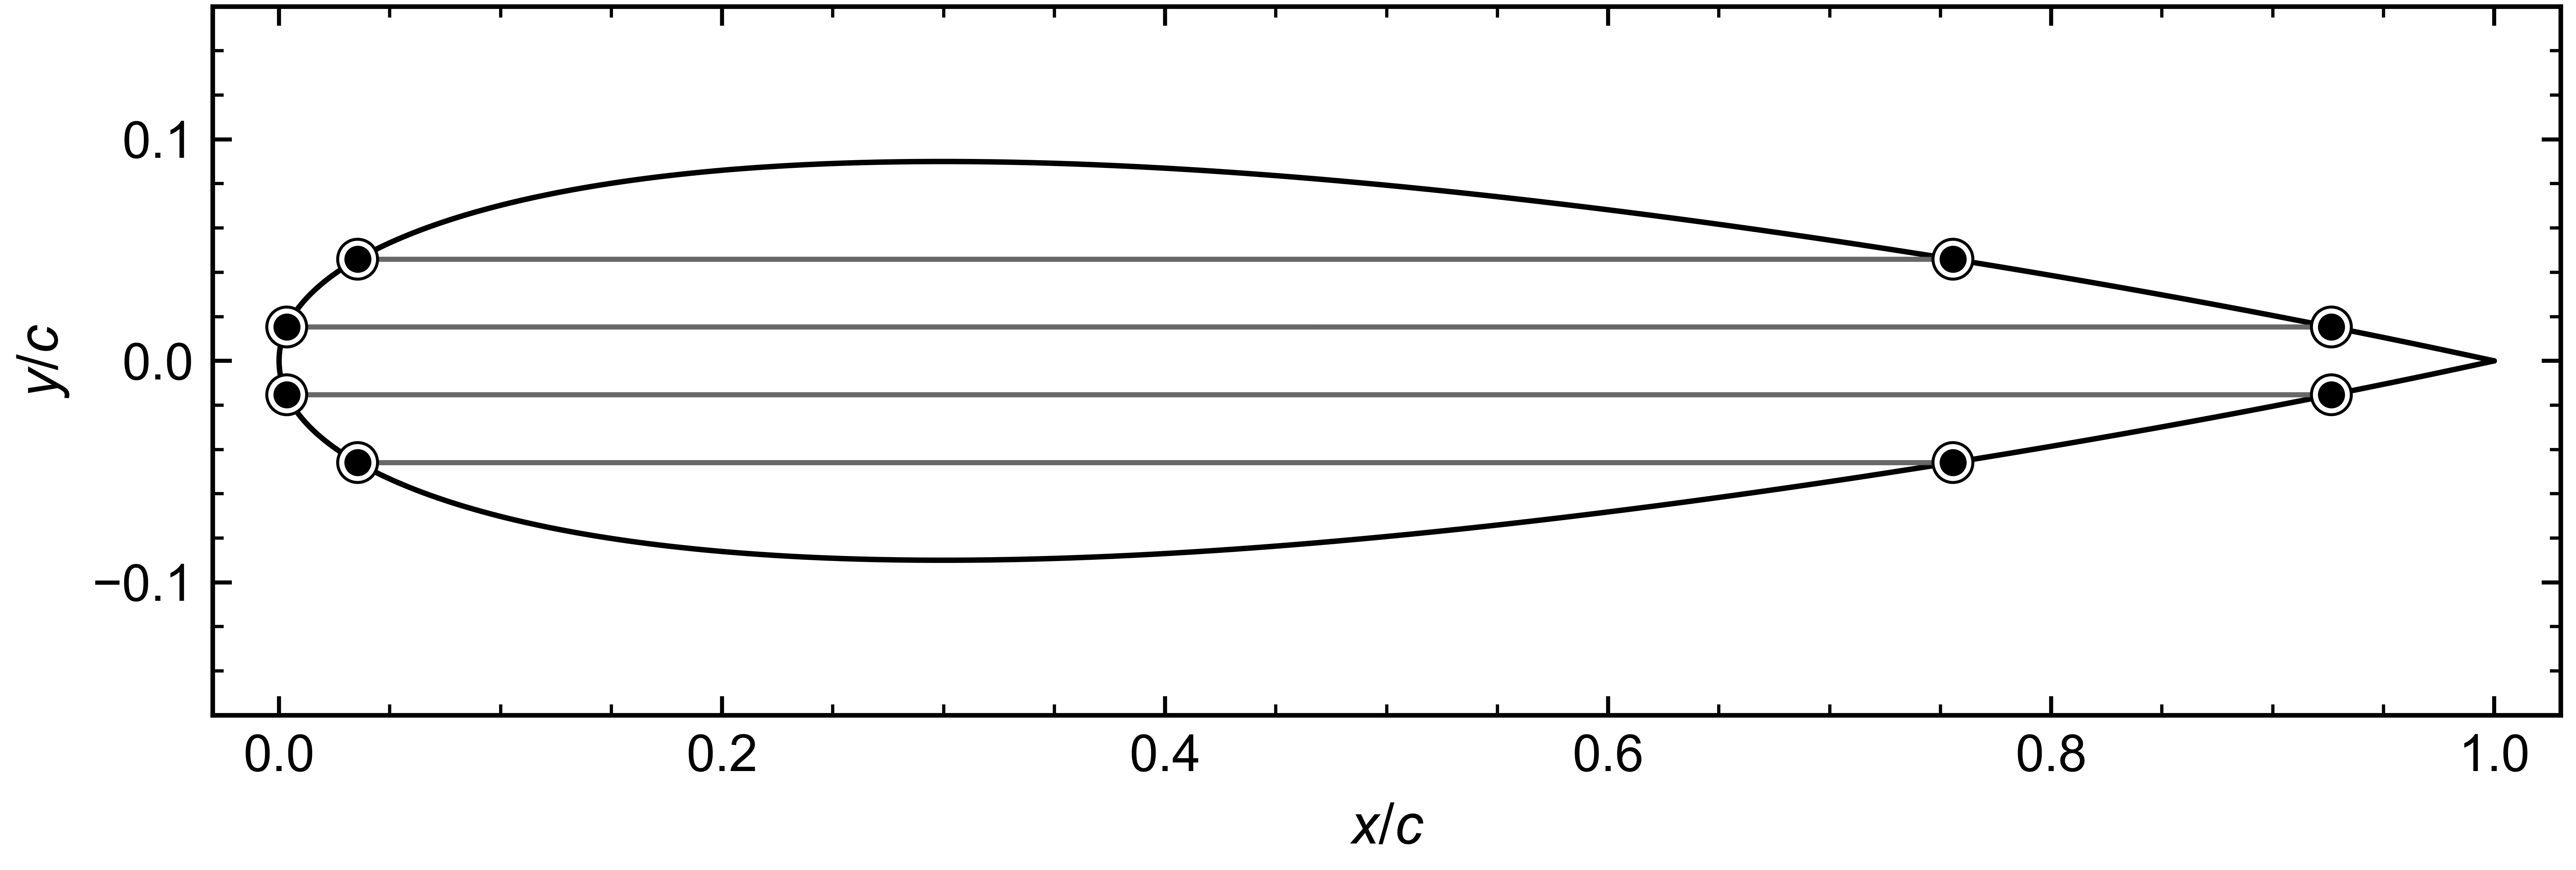
\includegraphics[
		width=0.80\linewidth,
		height=0.12\textheight,
		keepaspectratio
		]{figs/model1_horizontal.png}
		\par
		{\footnotesize\textbf{(a)} Chordwise layout\par}
		
		\vspace{2mm}
		
		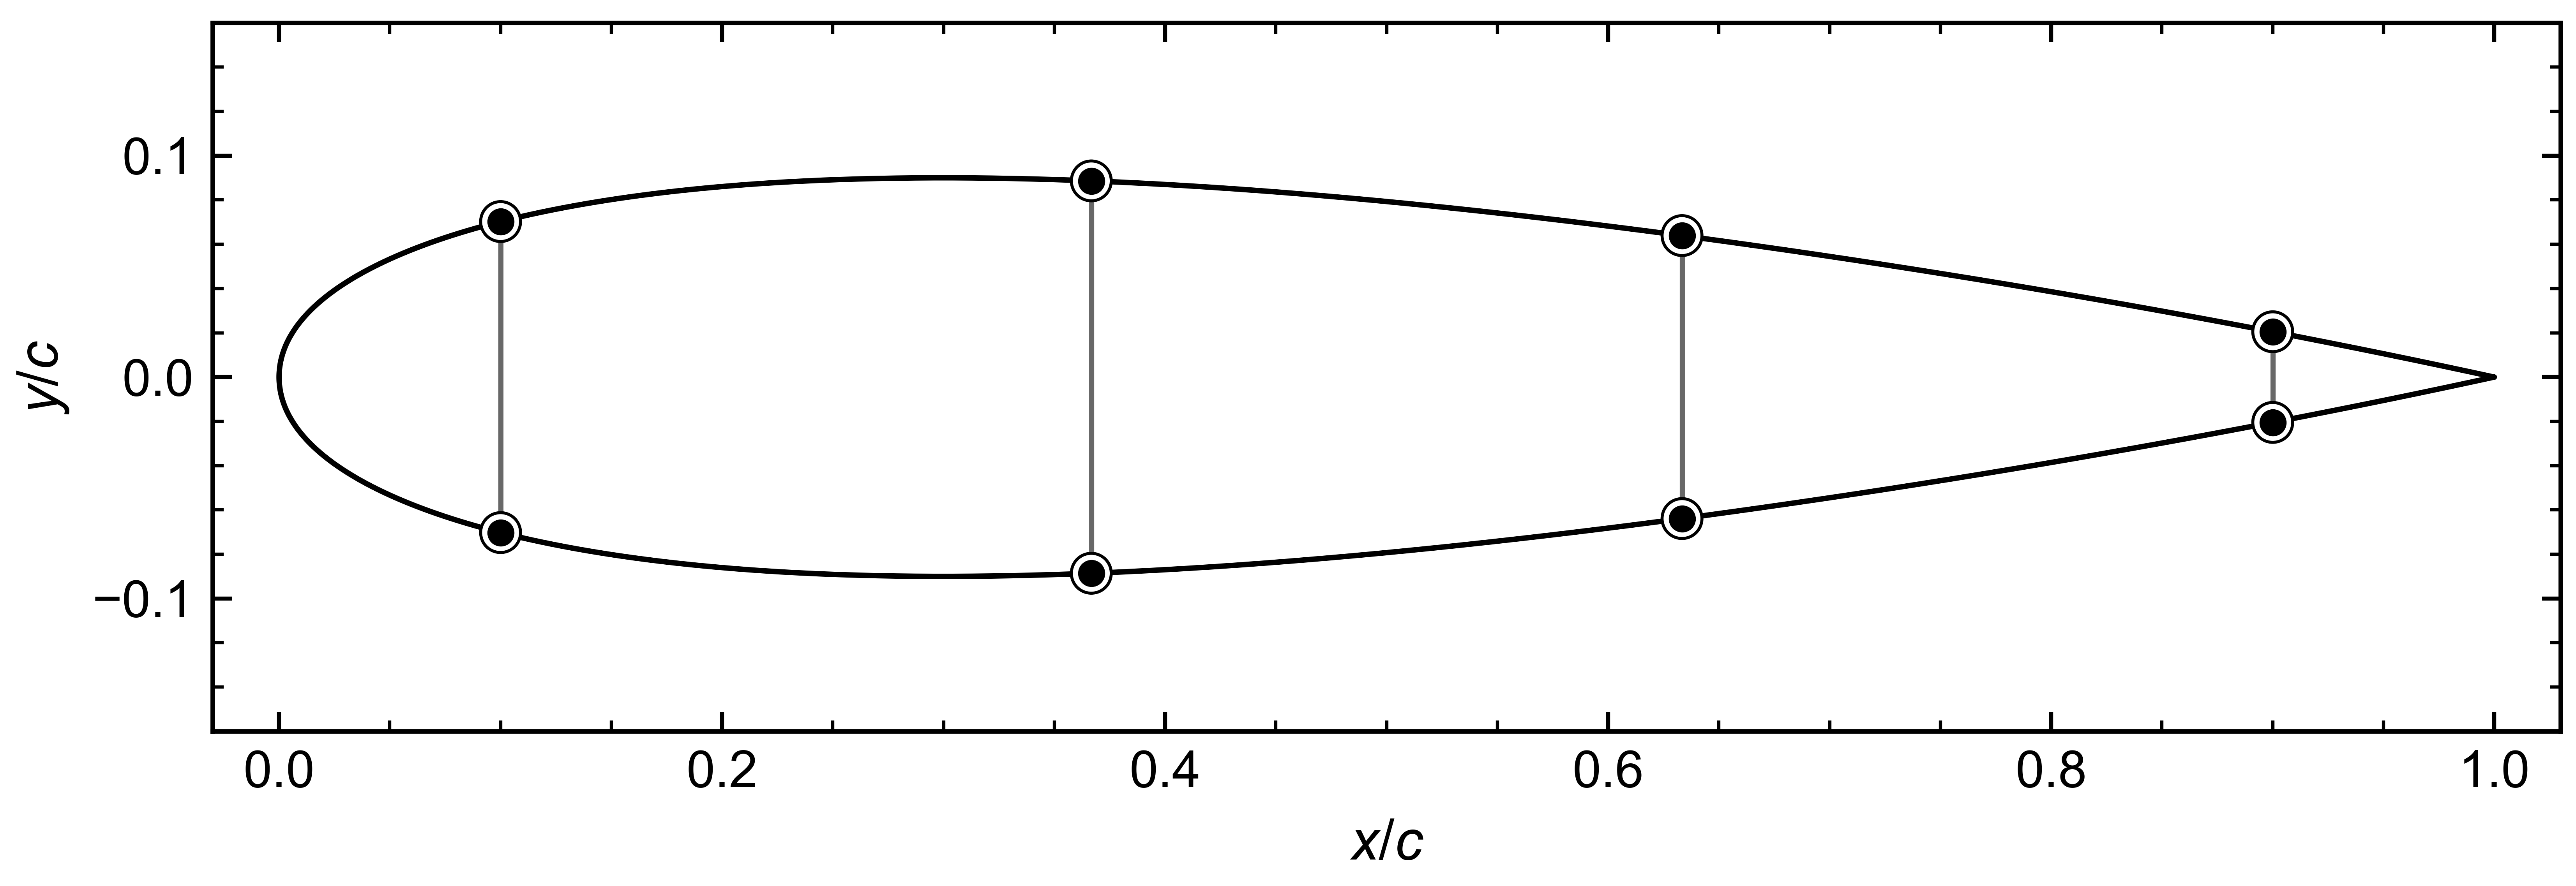
\includegraphics[
		width=0.80\linewidth,
		height=0.12\textheight,
		keepaspectratio
		]{figs/model2_vertical.png}
		\par
		{\footnotesize\textbf{(b)} Cross-surface layout\par}
		
		\vspace{2mm}
		
		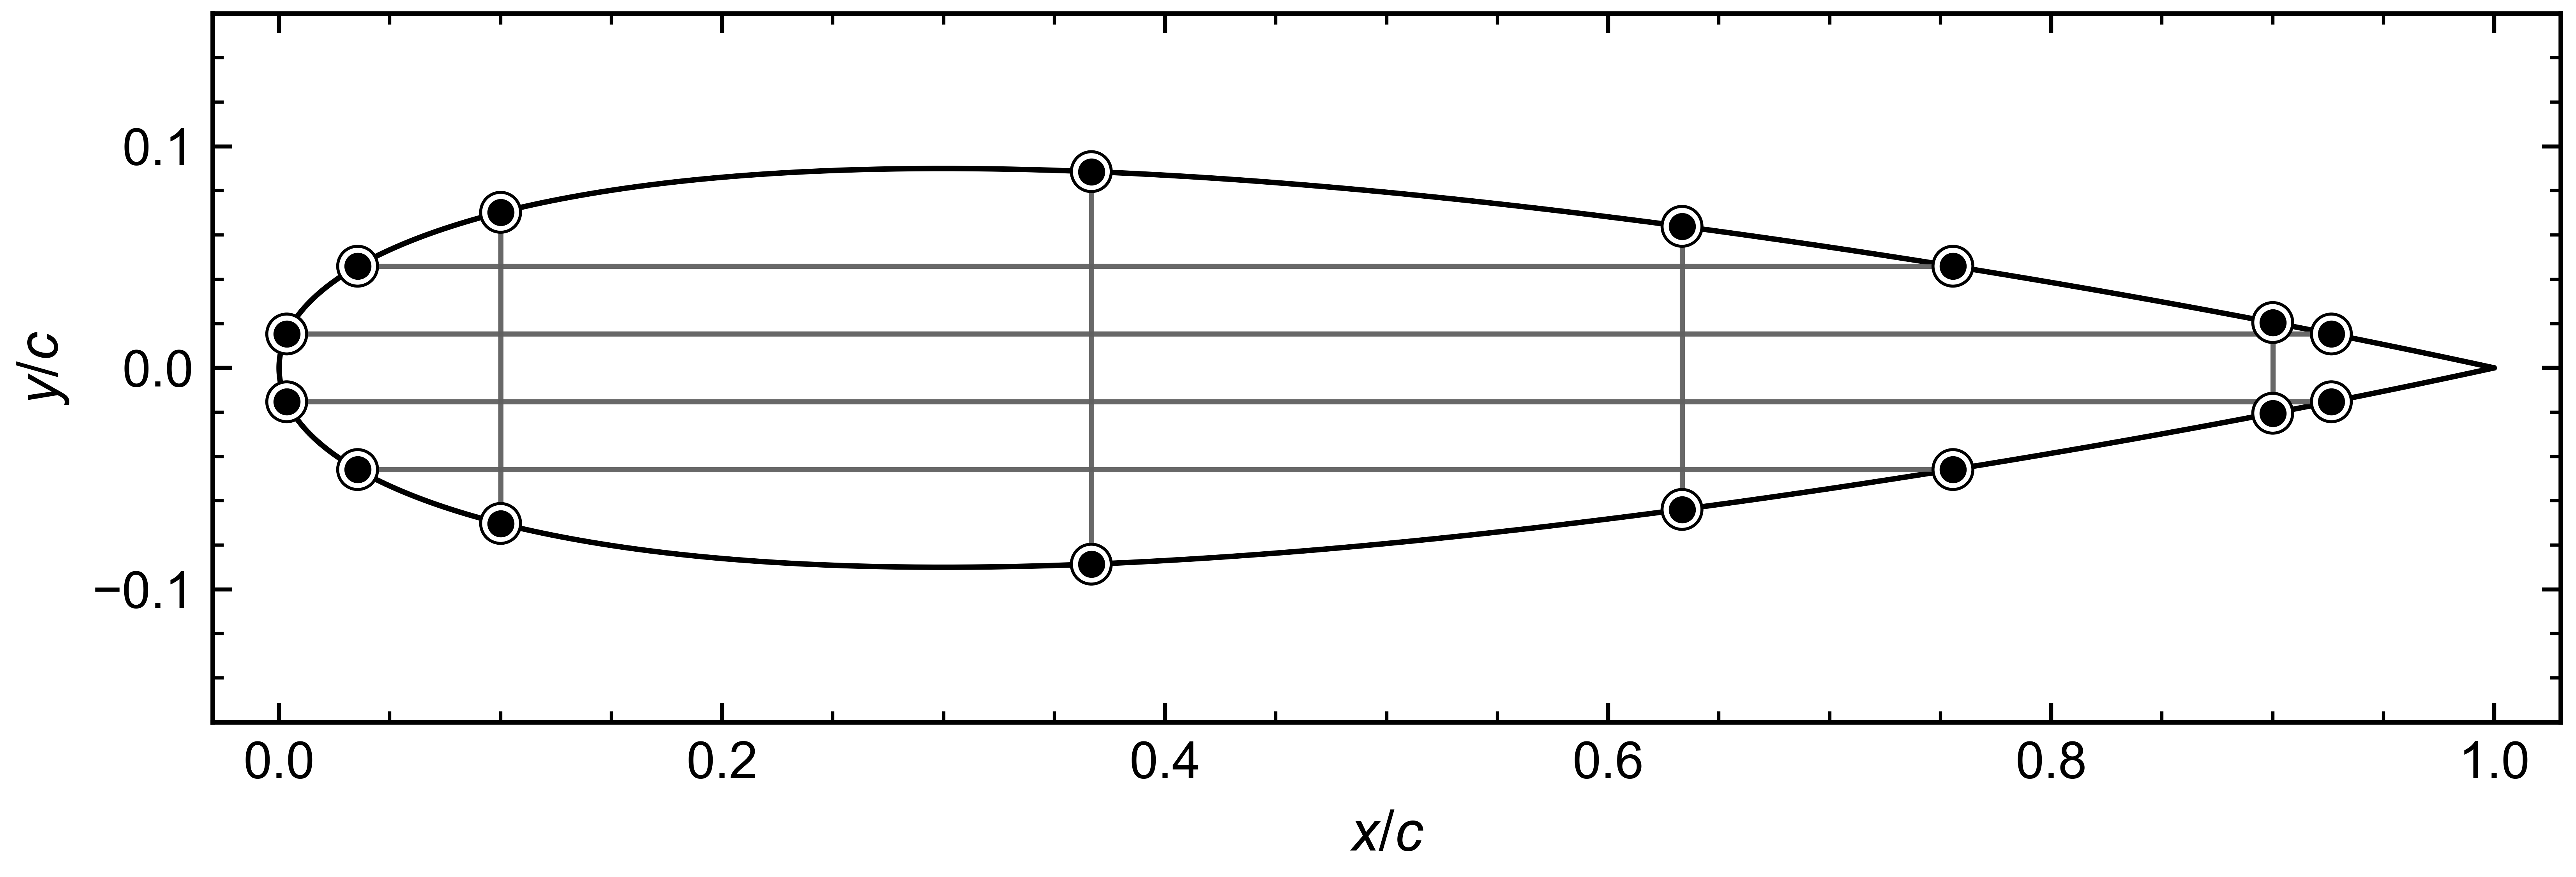
\includegraphics[
		width=0.80\linewidth,
		height=0.12\textheight,
		keepaspectratio
		]{figs/model3_combined.png}
		\par
		{\footnotesize\textbf{(c)} Combined independent layout\par}
		
		\caption{Internal-channel layouts considered in this study.}
		\label{fig:porous_models}
	\end{figure}
	
	
	Each pore is specified by a chordwise fraction, a surface identifier and the
	channel height $H_k$. The requested location is mapped to the polygonal airfoil
	surface independently of the panel control points. The channel centreline length
	$L_k$ is the straight-line distance between its two mapped surface endpoints.
	Before solution, the geometry is checked to ensure that every pore lies within
	the permitted chordwise range, that different pores do not overlap, that the
	specified minimum separation is maintained and that the channel fits within the
	local airfoil thickness. A geometry that fails any check is classified as invalid
	and is not included as a converged aerodynamic case.
	
	\subsection{External aerodynamic model}
	\label{subsec:external_aerodynamic_model}
	
	\subsubsection{Source--vortex panel formulation}
	
	The panel method follows the boundary-integral representation of incompressible
	potential flow developed by Hess and Smith and described in later panel-method
	treatments \cite{HessSmith1967PotentialFlow,KatzPlotkin2001LowSpeedAerodynamics,
		Birk2022HessSmithGuide}. With
	\begin{equation}
		\boldsymbol V=\nabla\Phi,
		\qquad \nabla^2\Phi=0,
		\label{eq:potential_flow}
	\end{equation}
	the external velocity is represented by the freestream, one constant source
	strength $\lambda_j$ on every panel and one uniform vortex-sheet strength
	$\gamma$ over the closed boundary. The sources represent thickness, while the
	vortex sheet provides the circulation required for a lifting solution.
	
	For a solid surface, the normal velocity at every control point is zero. At a
	pore, this boundary condition is replaced by a prescribed normal transpiration
	velocity, an approach consistent with reduced porous-surface formulations
	\cite{Hajian2017PorosityGradients,Baddoo2021UnsteadyPorousAerofoils}:
	\begin{equation}
		\boldsymbol V_i\boldsymbol\cdot\boldsymbol n_i=v_{n,i},
		\label{eq:transpiration_bc}
	\end{equation}
	where $v_{n,i}>0$ denotes flow out of the airfoil and $v_{n,i}<0$ denotes flow
	into it. With the adopted influence-coefficient convention, the discrete normal
	equation is
	\begin{equation}
		\pi\lambda_i+
		\sum_{\substack{j=1\\j\neq i}}^N I_{ij}\lambda_j
		-\gamma\sum_{j=1}^N K_{ij}
		=-2\pi V_\infty\cos\beta_i+2\pi v_{n,i},
		\label{eq:panel_normal_equation}
	\end{equation}
	where $I_{ij}$ and $K_{ij}$ are the normal source and vortex influence
	coefficients and $\beta_i$ is the angle between the panel normal and the
	freestream direction. The trailing-edge Kutta condition is
	\begin{equation}
		V_{t,1}+V_{t,N}=0.
		\label{eq:kutta_condition}
	\end{equation}
	Equations~\eqref{eq:panel_normal_equation} and \eqref{eq:kutta_condition} form an
	$(N+1)\times(N+1)$ linear system for
	$[\lambda_1,\ldots,\lambda_N,\gamma]^{\mathrm T}$. Because the influence matrix
	depends only on geometry, it is assembled and LU-factorised once for each airfoil
	discretisation; only the right-hand side changes when $\alpha$ or
	$\boldsymbol v_n$ changes.
	
	\subsubsection{Surface velocity and pressure}
	
	After solution of the panel system, the tangential velocity on panel $i$ is
	\begin{equation}
		V_{t,i}=V_\infty\sin\beta_i
		+\frac{1}{2\pi}\sum_{j=1}^N\lambda_jJ_{ij}
		+\frac{\gamma}{2}
		-\frac{\gamma}{2\pi}\sum_{j=1}^N L_{ij},
		\label{eq:tangential_velocity}
	\end{equation}
	where $J_{ij}$ and $L_{ij}$ are the tangential source and vortex influence
	coefficients. The prescribed normal component is retained when Bernoulli's
	equation is evaluated at a pore:
	\begin{equation}
		C_{p,i}=1-\frac{V_{t,i}^2+v_{n,i}^2}{V_\infty^2},
		\qquad
		p_i=p_\infty+\frac{1}{2}\rho_\infty V_\infty^2C_{p,i}.
		\label{eq:panel_pressure}
	\end{equation}
	This expression is a potential-flow closure at the exterior surface; it does not
	resolve the dissipative pore-mouth region.
	
	\subsection{Internal rectangular-channel model}
	\label{subsec:internal_channel_model}
	
	Channel $k$ is treated as a two-dimensional rectangular duct of height $H_k$
	and length $L_k$, with all flow quantities expressed per unit span. The signed
	flow rate per unit span $q'_k$, positive from labelled pore 1 to labelled pore 2,
	and bulk velocity $U_k$ are related by
	\begin{equation}
		U_k=\frac{q'_k}{H_k},
		\qquad D_{h,k}=2H_k,
		\qquad
		Re_{h,k}=\frac{\rho_\infty |U_k|D_{h,k}}{\mu_\infty}.
		\label{eq:channel_kinematics}
	\end{equation}
	The Darcy--Weisbach friction loss is
	\begin{equation}
		\Delta p_{f,k}=f_k\frac{L_k}{D_{h,k}}
		\frac{\rho_\infty U_k^2}{2}.
		\label{eq:channel_friction_loss}
	\end{equation}
	For $Re_{h,k}\leq2000$, the parallel-wall result
	$f_k=96/Re_{h,k}$ is used \cite{ShahLondon1978LaminarDucts}; substitution into
	Eq.~\eqref{eq:channel_friction_loss} gives the plane-Poiseuille limit
	\begin{equation}
		\Delta p_{f,k}=\frac{12\mu_\infty L_k}{H_k^2}|U_k|,
		\qquad
		R'_k=\frac{\Delta p_{f,k}}{|q'_k|}
		=\frac{12\mu_\infty L_k}{H_k^3}.
		\label{eq:parallel_wall_limit}
	\end{equation}
	For $Re_{h,k}\geq3000$, the adopted smooth-wall approximation is
	$f_k=0.3164Re_{h,k}^{-1/4}$. This pipe-flow correlation is extended to the
	parallel-wall channel using its hydraulic diameter and is not a geometry-specific
	turbulent-channel validation. The Darcy friction-factor convention is used
	throughout \cite{Moody1944FrictionFactors}. A continuously differentiable blend
	is applied between the two limits:
	\begin{align}
		\xi_k&=\frac{Re_{h,k}-2000}{1000},
		&w_k&=\xi_k^2(3-2\xi_k),\nonumber\\
		f_k&=(1-w_k)\frac{96}{Re_{h,k}}
		+w_k\frac{0.3164}{Re_{h,k}^{1/4}}.
		\label{eq:friction_blend}
	\end{align}
	The blended relation is an engineering closure used to avoid a discontinuity;
	it is not a transition model for the developing pore flow.
	
	Let $p_{\mathrm{in},k}$ and $p_{\mathrm{out},k}$ denote the area-averaged static
	pressures at the higher- and lower-pressure pores, respectively. The active
	energy closure is
	\begin{equation}
		p_{\mathrm{in},k}-p_{\mathrm{out},k}
		+\left\langle\frac{1}{2}\rho_\infty v_n^2\right\rangle_{\mathrm{in},k}
		=\Delta p_{f,k}
		+\alpha_j\frac{1}{2}\rho_\infty U_k^2,
		\label{eq:channel_energy_closure}
	\end{equation}
	with $\alpha_j=1$. The external tangential kinetic head is assumed to be lost
	during turning into the channel and is therefore not credited as available
	channel head. At the outlet, the static pressure is matched to the exterior,
	while the bulk jet kinetic head is carried out of the channel. Equation
	\eqref{eq:channel_energy_closure} is monotonic in $|U_k|$ and is solved by a
	bracketed scalar bisection. The flow direction is taken from the sign of the
	static pore-pressure difference; an exact pressure tie gives zero flow. This
	closure assumes zero recovery of inlet tangential kinetic energy; it has not been calibrated against a
	resolved three-dimensional pore-mouth flow and should be interpreted as a
	reduced-order modelling assumption.
	
	\subsection{Pore averaging and aero--hydraulic coupling}
	\label{subsec:aero_hydraulic_coupling}
	
	\subsubsection{Pressure averaging and flow transfer}
	
	The intersection of a channel strip with the polygonal surface defines the
	finite extent of each pore. Surface pressure is reconstructed piecewise linearly
	through panel-centre values and integrated along the pore. Thus, for pore $m$ of
	channel $k$,
	\begin{equation}
		p_{m,k}=\frac{1}{\ell_{m,k}}
		\int_{\mathcal P_{m,k}}p(s)\,\mathrm ds,
		\qquad
		\ell_{m,k}=\int_{\mathcal P_{m,k}}\mathrm ds.
		\label{eq:pore_pressure_average}
	\end{equation}
	This treatment allows a pore boundary to cut through a panel without moving the
	prescribed physical location.
	
	The channel flow is transferred to the intersected panels as a panel-average
	normal velocity. If $\ell_{i,m,k}$ is the portion of panel $i$ covered by pore
	$m$ of channel $k$, then
	\begin{equation}
		v_{n,i}^{(m,k)}=\sigma_{m,k}
		\frac{q'_k\ell_{i,m,k}}{\ell_{m,k}S_i},
		\qquad
		\sigma_{m,k}=\begin{cases}-1,&m=1,\\+1,&m=2.
		\end{cases}
		\label{eq:conservative_pore_mapping}
	\end{equation}
	Consequently,
	\begin{equation}
		\sum_{i\in\mathcal P_{m,k}}v_{n,i}^{(m,k)}S_i
		=\sigma_{m,k}q'_k,
		\label{eq:pore_mass_conservation}
	\end{equation}
	For $q'_k>0$, pore 1 is the inlet and pore 2 is the outlet; these roles reverse
	when $q'_k<0$. Thus each independently connected channel conserves flow exactly within the
	two-dimensional per-unit-span formulation. Contributions are summed if more than
	one channel acts on the aerodynamic boundary, although overlapping pores are
	excluded by the geometry checks.
	
	\subsubsection{Nonlinearity and solution procedure}
	\label{subsubsec:nonlinear_coupling}
	
	The panel equations are linear when the pore-normal velocities are prescribed.
	The coupled problem is nonlinear because these velocities depend on channel
	flow rates driven by the pressure distribution they produce. Pressure depends
	on squared velocity through Bernoulli's equation, while the channel model
	includes a Reynolds-number-dependent friction factor and an outlet kinetic-head
	term. Directly repeating pressure and flow updates can therefore oscillate or
	fail to converge. Larger channels can strengthen this feedback because the
	laminar hydraulic resistance decreases as $H_k^{-3}$.
	
	To obtain a consistent solution, all channel flow rates are solved together
	as a nonlinear root problem. The dimensionless unknowns are
	\begin{equation}
		\widehat q_k=\frac{q'_k}{H_kV_\infty}.
	\end{equation}
	For a trial vector, the panel solver and channel model return the pressure-driven
	flow vector $\boldsymbol q'_{\mathrm{hyd}}$. The residual is
	\begin{equation}
		R_k(\widehat{\boldsymbol q})=
		\frac{q'_{k,\mathrm{trial}}-q'_{k,\mathrm{hyd}}}{H_kV_\infty}.
		\label{eq:coupling_residual}
	\end{equation}
	A Powell hybrid root solver adjusts the trial flows to reduce this mismatch,
	with a trust-region reflective least-squares method used if required
	\cite{MoreGarbowHillstrom1980MINPACK,Virtanen2020SciPy}. Each trial requires a
	linear panel solve followed by the channel-flow calculation. A solution is
	accepted only when the scaled residual satisfies
	\begin{equation}
		\|\boldsymbol R\|_\infty\leq
		\sqrt{\epsilon_{\mathrm{mach}}}
		\max\left(1,\|\widehat{\boldsymbol q}\|_\infty\right).
		\label{eq:coupling_tolerance}
	\end{equation}
	
	where $\epsilon_{\mathrm{mach}}$ is machine precision. A successful solver
	termination alone is insufficient if this condition is not met.
	
	The angle-of-attack sweep begins at the requested angle nearest to zero and
	advances towards positive and negative angles, using converged channel flows
	to initialise neighbouring cases. For difficult cases, continuation introduces
	intermediate operating conditions or gradually increases the coupling strength.
	The available strategies include adaptive angle steps, Reynolds-number
	continuation where applicable, coupling homotopy and pseudo-arclength
	continuation. Only solutions satisfying the fully coupled equations at the
	requested operating conditions are retained. Invalid geometries are rejected
	before solution, and cases that remain unconverged after the available attempts
	are reported as \texttt{NaN}. Non-convergence does not establish stall or prove
	that no steady solution exists.
	
	\subsection{Aerodynamic output coefficients}
	\label{subsec:aerodynamic_coefficients}
	
	Pressure forces are integrated over the closed polygonal boundary:
	\begin{align}
		\mathrm dC_{x,i}&=-C_{p,i}n_{x,i}\frac{S_i}{c},&
		\mathrm dC_{y,i}&=-C_{p,i}n_{y,i}\frac{S_i}{c},\nonumber\\
		C_x&=\sum_{i=1}^N\mathrm dC_{x,i},&
		C_y&=\sum_{i=1}^N\mathrm dC_{y,i}.
		\label{eq:cartesian_pressure_forces}
	\end{align}
	The freestream-aligned coefficients are
	\begin{align}
		C_L&=C_y\cos\alpha-C_x\sin\alpha,\nonumber\\
		C_{D,p}&=C_x\cos\alpha+C_y\sin\alpha.
		\label{eq:lift_pressure_drag}
	\end{align}
	Here $C_{D,p}$ is a closed-contour pressure-based streamwise-force coefficient;
	it is not total drag because skin friction and viscous wake momentum loss are not
	included. In addition, the integration retains pressure on the nominal contour
	across the pores and does not explicitly include internal-wall forces or the
	momentum transported through the pores. It must therefore not be identified with
	the net force on the complete porous device. The same qualification applies to
	the pressure-integrated lift and moment. The quarter-chord pitching-moment coefficient is
	\begin{equation}
		C_M=-\sum_{i=1}^N
		\frac{(x_i-0.25c)\,\mathrm dC_{y,i}-y_i\,\mathrm dC_{x,i}}{c}.
		\label{eq:pitching_moment}
	\end{equation}
	As an internal check, a circulation-based lift coefficient is also evaluated:
	\begin{equation}
		C_{L,\Gamma}=\frac{2\gamma\sum_{i=1}^NS_i}{V_\infty c}.
		\label{eq:circulation_lift}
	\end{equation}
	
	\subsection{Numerical conditions and verification}
	\label{subsec:numerical_setup}
	
	The conditions used for the reported study are listed in
	Table~\ref{tab:numerical_setup}. The freestream speed is calculated from
	\begin{equation}
		V_\infty=\frac{Re_c\mu_\infty}{\rho_\infty c}.
		\label{eq:freestream_velocity}
	\end{equation}
	
	\begin{table}
		\centering
		\caption{Numerical and operating conditions used in the present study.}
		\label{tab:numerical_setup}
		\begin{tabular}{lll}
			\hline
			\textbf{Parameter} & \textbf{Symbol} & \textbf{Value}\\
			\hline
			Airfoil & -- & NACA~0018\\
			Chord length & $c$ & $1~\mathrm{m}$\\
			Number of panels & $N$ & $1000$\\
			Fluid density & $\rho_\infty$ & $1.225~\mathrm{kg\,m^{-3}}$\\
			Dynamic viscosity & $\mu_\infty$ & $1.8\times10^{-5}~\mathrm{Pa\,s}$\\
			Freestream pressure & $p_\infty$ & $101325~\mathrm{Pa}$\\
			Chord Reynolds number & $Re_c$ & $5.0\times10^5$\\
			Principal angle of attack & $\alpha$ & $4^\circ$\\
			Angle-of-attack range & $\alpha$ & $-5^\circ$ to $15^\circ$\\
			Angle increment & $\Delta\alpha$ & $1^\circ$\\
			Channel height & $H$ & $8,\;9,\;10~\mathrm{mm}$\\
			\hline
		\end{tabular}
	\end{table}
	
	The impermeable airfoil is solved with the same geometry, panel distribution and
	operating conditions as the channelled configurations. An inviscid XFOIL
	solution, based on a linear-vorticity panel method, is used as an independent
	reference for the impermeable-airfoil surface-pressure distribution and
	angle-of-attack trend \cite{Drela1989XFOIL}. This comparison is a verification of
	the external-flow implementation and does not validate the internal channel or
	pore-mouth closures.
	
	% AUTHOR CHECK: insert the completed panel-refinement study and its quantitative
	% acceptance criterion here. Do not claim grid independence without those results.
	A panel-refinement assessment is required for the impermeable airfoil and
	representative coupled cases, monitoring $C_p$, $C_L$, $C_{D,p}$, $C_M$ and
	channel flow rates. The nominal production value is $N=1000$; convergence of
	integrated forces alone does not establish convergence of local pore pressures.
	For every coupled case, available diagnostics include the panel-system residual,
	Kutta residual, normal-boundary-condition residual, channel energy residual,
	maximum $|v_n|/V_\infty$, hydraulic Reynolds number and nonlinear coupling
	residual. These checks distinguish numerical convergence from the physical
	limitations of the reduced-order model.
	
	% Keep Methods figures and table before Results.
	\FloatBarrier
	
	\section{Results and discussion}
	\label{sec:results_discussion}
	
	The aerodynamic behaviour of the three porous-airfoil configurations
	was investigated over an angle-of-attack range of $-5^\circ$ to
	$15^\circ$. Three pore heights, $H=8$, $9$ and $10~\mathrm{mm}$,
	were considered for the horizontal, vertical and horizontal--vertical
	porous airfoils. The corresponding impermeable (solid) airfoil
	panel-method solution and the inviscid XFOIL prediction are included as
	reference cases.
	
	The effect of the pores is first examined through the lift and
	moment coefficients over the angle-of-attack range. The observed aerodynamic trends are then
	interpreted using the corresponding pressure and velocity field
	differences. A detailed flow-field comparison is presented at
	$\alpha=10^\circ$ for a pore height of $H=9~\mathrm{mm}$.
	
	
	% ============================================================
	% BASELINE VALIDATION
	% ============================================================
	
	\subsection{Panel method validation against XFOIL}
	\label{subsec:Panel_method_validation_against_XFOIL}
	
	The impermeable source--vortex panel-method solution is compared with
	the corresponding inviscid XFOIL prediction in
	Figures.~\ref{fig:cl_aoa_three_models} and
	\ref{fig:cm_aoa_three_models}. Both methods show similar trends in lift
	and pitching moment over the investigated angle-of-attack range.
	
	This agreement provides a useful reference for assessing the aerodynamic
	effects introduced by the pores. Small differences between the
	panel-method and XFOIL predictions are expected because the two
	approaches use different numerical formulations, although both represent
	inviscid external flow.
	
	The impermeable panel-method solution is therefore used as the primary
	reference when evaluating the porous-airfoil configurations. This
	ensures that the porous and solid airfoils are compared using the same
	geometry, panel discretisation, aerodynamic formulation and operating
	conditions.
	
	% ============================================================
	% LIFT
	% ============================================================
	
	\subsection{Effect of pores on lift}
	\label{subsec:lift_results}
	
	Figure~\ref{fig:cl_aoa_three_models} compares the variation of lift
	coefficient with angle of attack for the three porous-airfoil
	configurations and pore heights.
	\begin{figure*}
		\centering
		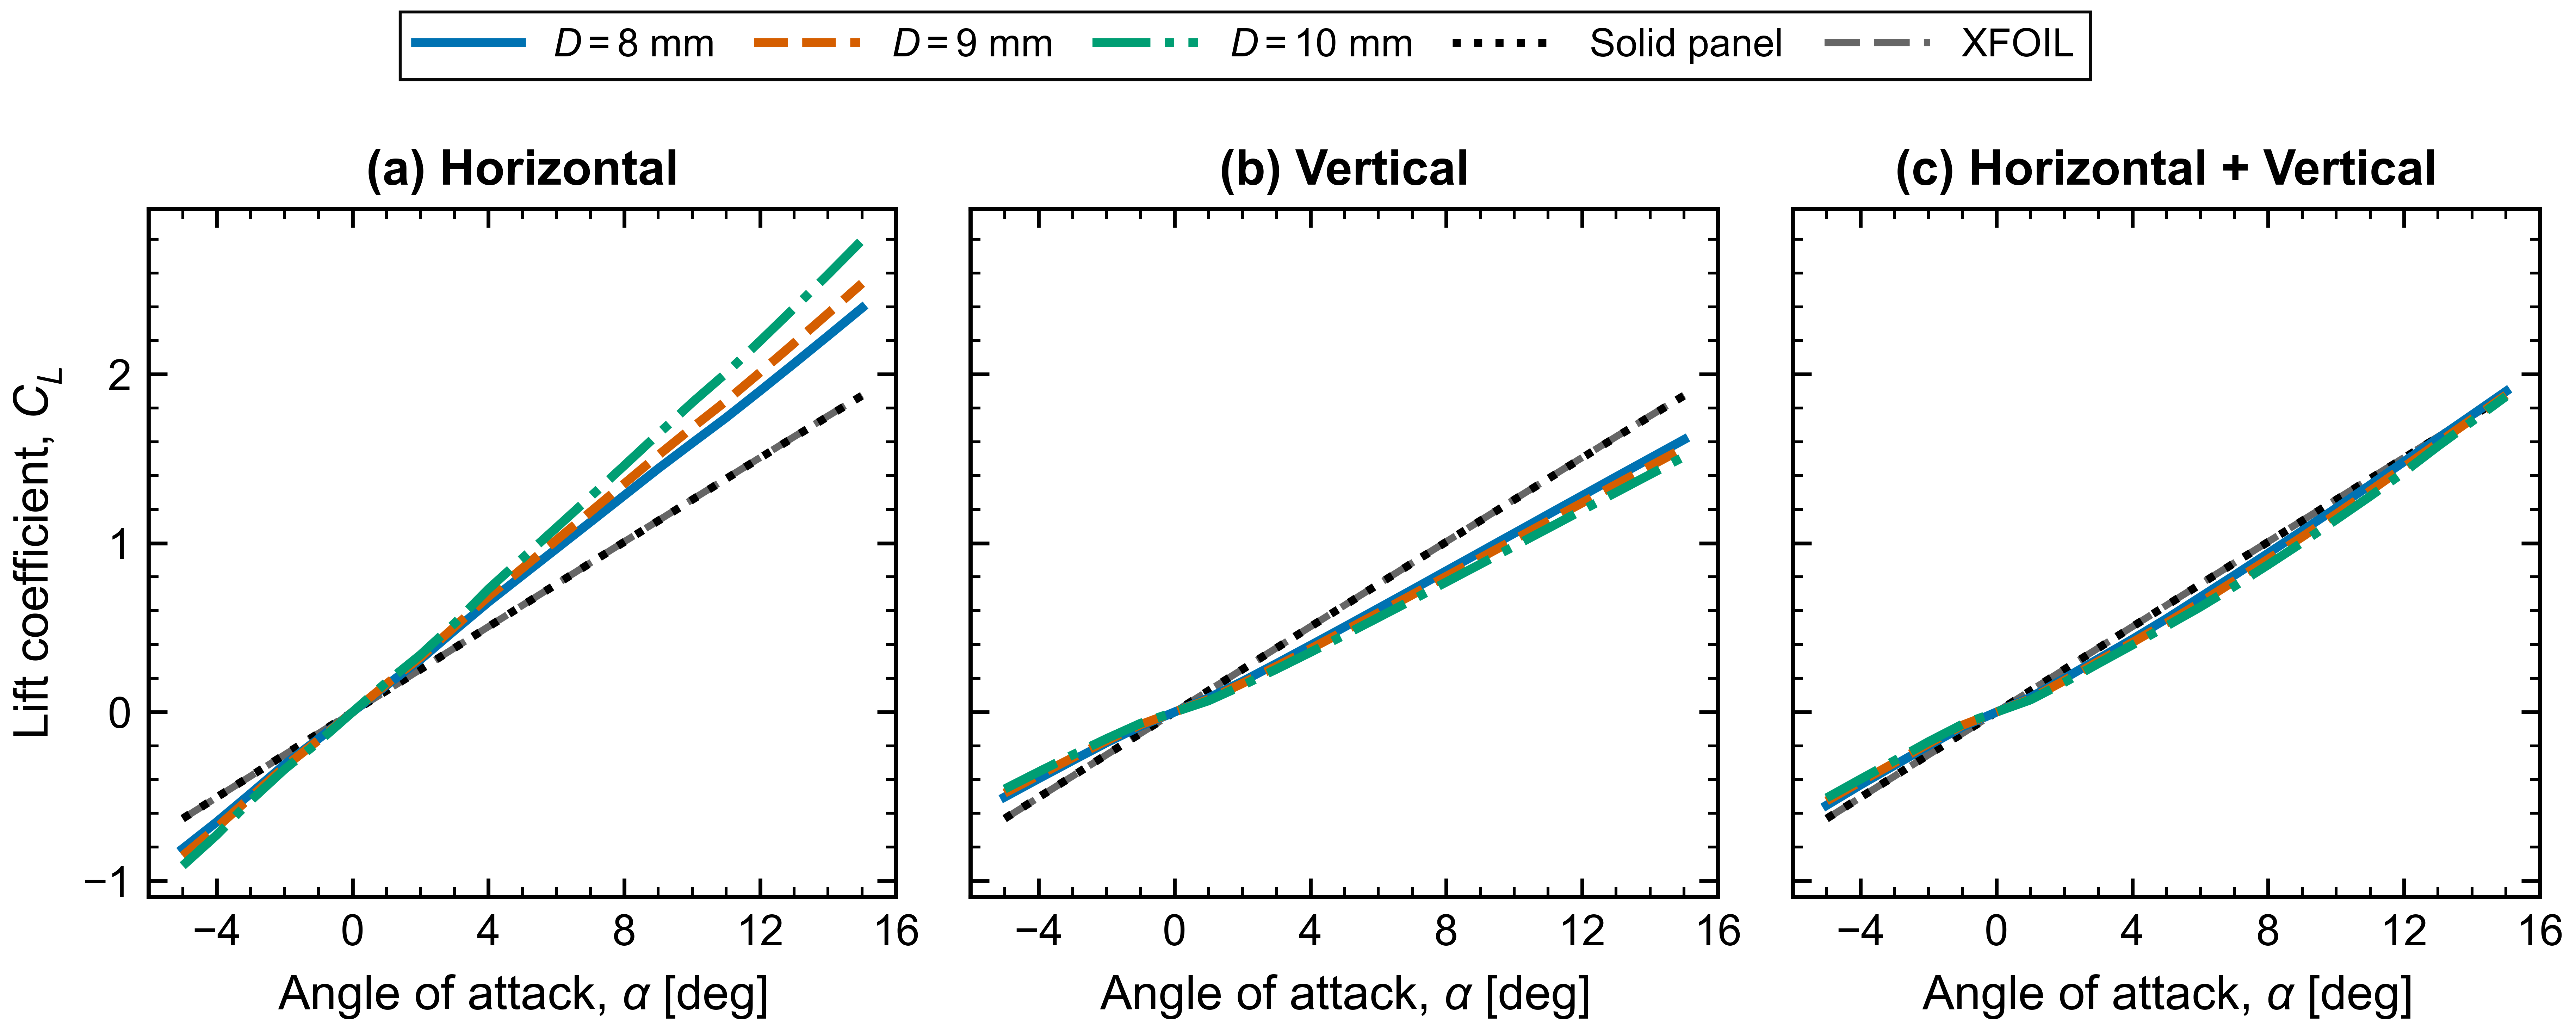
\includegraphics[
		width=0.96\textwidth
		]{figs/CL_vs_AoA_three_models_three_diameters.png}
		\caption{
			Lift coefficient as a function of angle of attack for
			(a) the horizontal porous airfoil,
			(b) the vertical porous airfoil, and
			(c) the horizontal--vertical porous airfoil.
			Results are shown for pore heights
			$H=8$, $9$ and $10~\mathrm{mm}$ together with the
			impermeable panel-method and inviscid XFOIL reference
			solutions.
		}
		\label{fig:cl_aoa_three_models}
	\end{figure*}
	The horizontal porous airfoil produces the largest change in lift.
	At positive angles of attack, its lift coefficient is higher than that
	of the impermeable reference, and the difference becomes more
	pronounced as the angle of attack increases. The effect also strengthens
	with pore height, with $H=10~\mathrm{mm}$ producing the highest lift
	at larger positive angles of attack. At negative angles of attack,
	increasing the pore height similarly increases the magnitude of the
	negative lift.This nearly symmetric lift response about the zero-lift condition is
	consistent with the symmetric NACA~0018 geometry.
	
	For the horizontal configuration, both ends of each pore are located on
	the same airfoil surface. The streamwise variation in surface pressure
	therefore creates a pressure difference between the two ends and drives
	internal flow from the locally higher-pressure region towards the
	lower-pressure region. This produces suction at one end and blowing at
	the other, changing the local surface-normal velocity and redistributing
	the external pressure and velocity fields along the airfoil surface.
	At positive angle of attack, the different pressure distributions over
	the suction and pressure surfaces lead to a net redistribution of
	aerodynamic loading that increases lift.
	
	The stronger dependence on pore height is consistent with the reduction
	in hydraulic resistance as the pore becomes larger. For a given pressure
	difference, a larger pore height permits a greater internal flow and
	therefore a stronger interaction between the pore flow and the external
	aerodynamic field.
	
	The vertical porous airfoil shows a distinctly different behaviour.
	At positive angles of attack, its lift coefficient is generally lower
	than that of the impermeable airfoil, while the three pore-height cases
	remain relatively close over most of the investigated range.
	
	In this configuration, each pore connects the  pressure
	surface to the suction surface. The resulting pressure
	difference drives internal flow between the two surfaces and partially
	reduces the pressure difference responsible for lift. This pressure
	equalisation is consistent with the lower lift coefficient obtained for
	the vertical porous airfoil. The small separation between the
	pore-height cases also indicates that this configuration is less
	sensitive to pore height than the horizontal arrangement.
	
	The horizontal--vertical porous airfoil remains comparatively close to
	the impermeable reference. At positive angles of attack, its lift
	coefficient is generally slightly lower than that of the solid airfoil,
	and the three pore-height cases remain closely grouped.
	
	This behaviour reflects the simultaneous influence of the horizontal
	and vertical pore arrangements. The horizontal pores redistribute flow
	between different chordwise locations on the same surface, whereas the
	vertical pores transfer flow between the pressure and suction surfaces.
	The lift-enhancing redistribution associated with the horizontal pores
	is therefore partly offset by the pressure equalisation introduced by
	the vertical pores.
	
	The horizontal and vertical pores remain physically separate and
	hydraulically independent. However, their aerodynamic effects interact
	through the external pressure field, since changes produced by one set
	of pores alter the surface pressures that drive the other set.
	Consequently, the response of the horizontal--vertical porous airfoil is
	not a simple superposition of the two individual configurations.
	
	Overall, the results show that the aerodynamic effect of the pores is
	governed mainly by their orientation, placement and the pressure
	difference between the connected surface locations. Pore height also
	influences the response, but its effect is strongest for the horizontal
	configuration and considerably weaker for the vertical and
	horizontal--vertical arrangements.
	% ============================================================
	% PITCHING MOMENT
	% ============================================================
	
	\subsection{Effect of pores on pitching moment}
	\label{subsec:moment_results}
	
	The corresponding moment coefficients are
	presented in Figure.~\ref{fig:cm_aoa_three_models}.
	\begin{figure*}
		\centering
		
		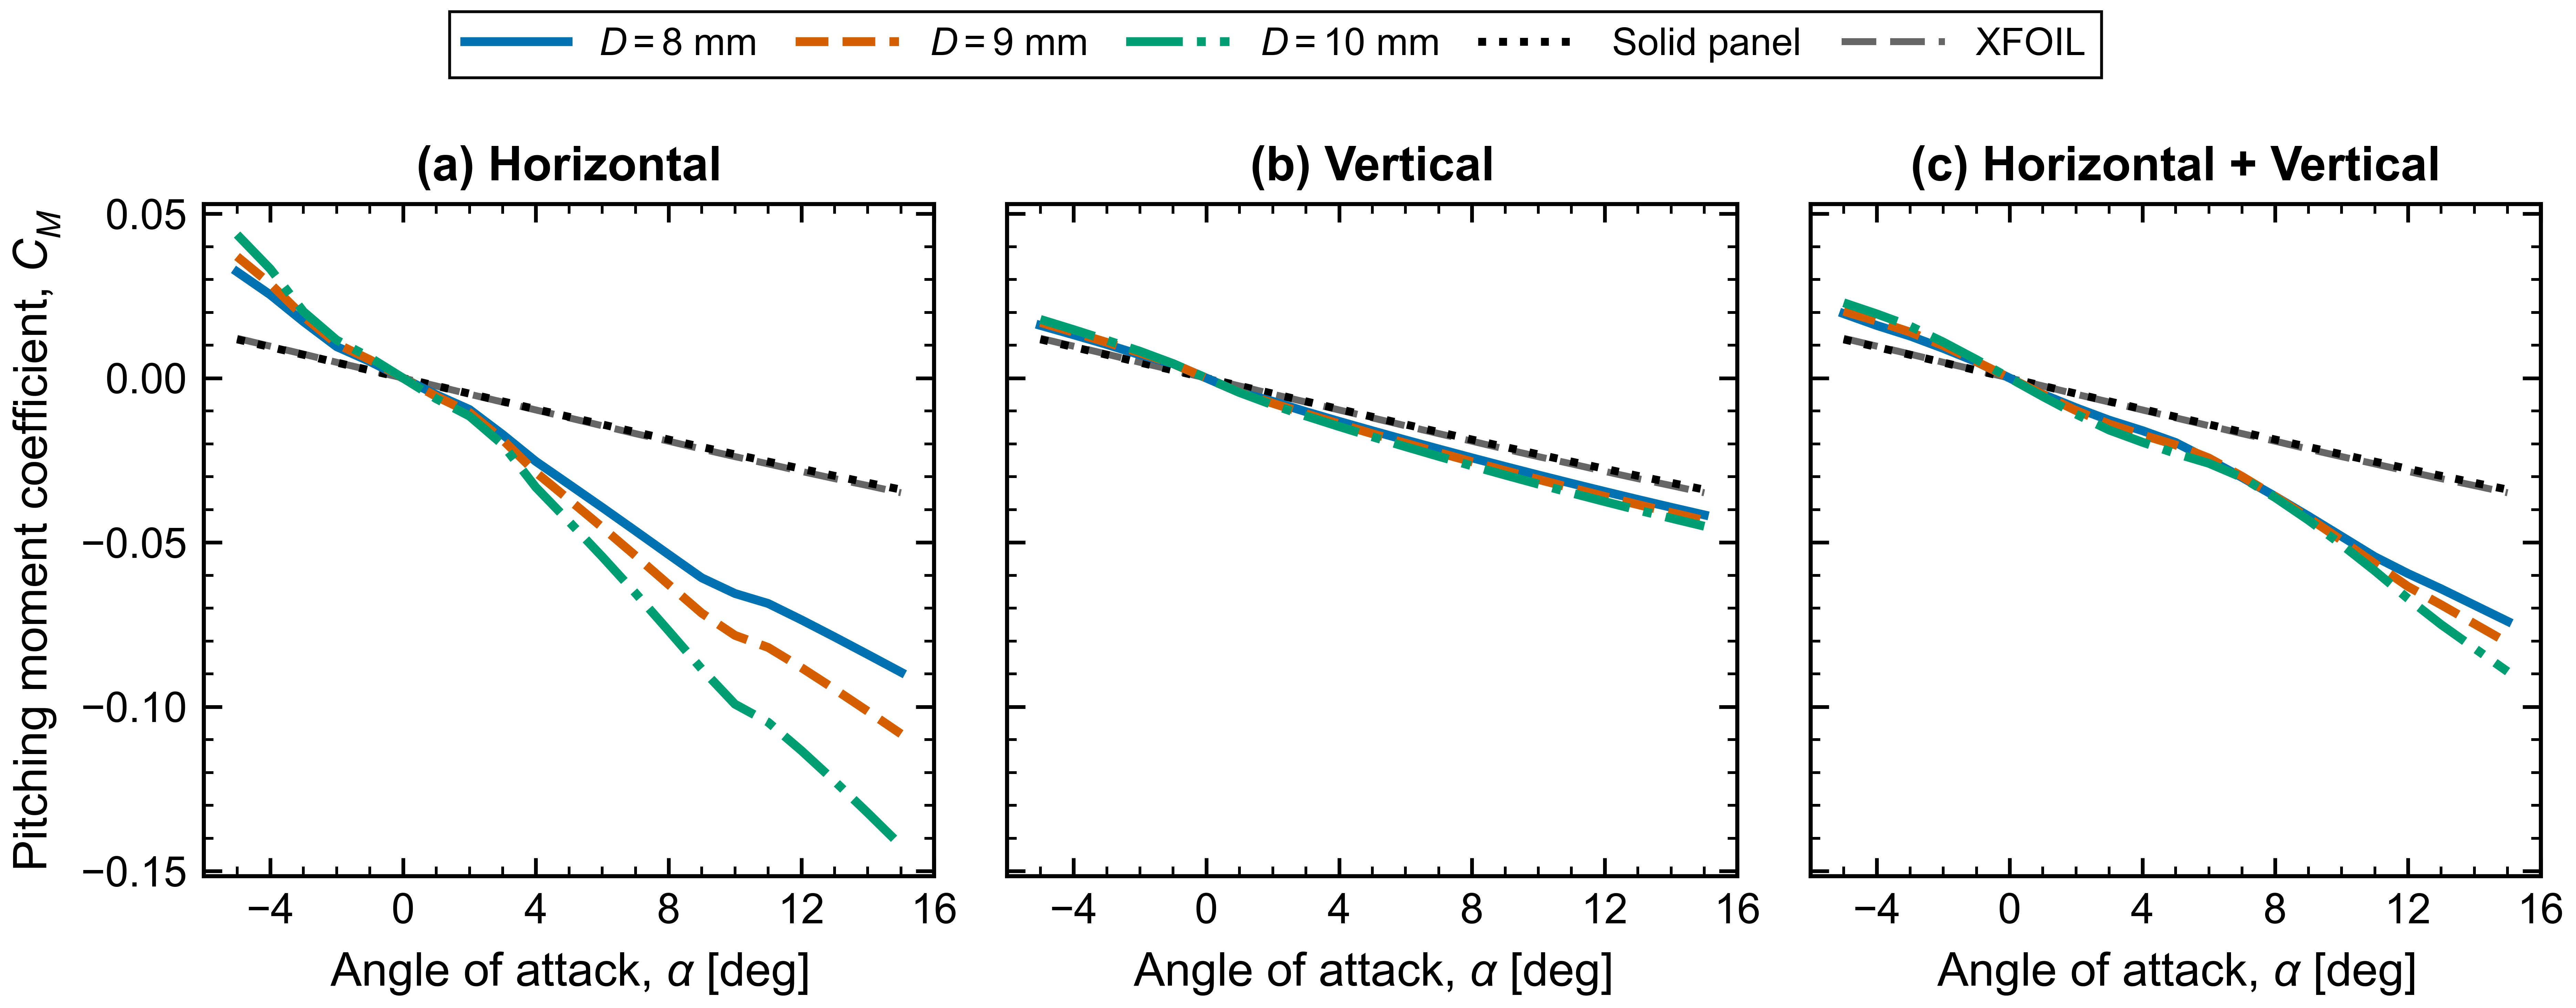
\includegraphics[
		width=0.96\textwidth
		]{figs/CM_vs_AoA_three_models_three_diameters.png}
		
		\caption{
			Pitching-moment coefficient about the quarter chord as a
			function of angle of attack for
			(a) the horizontal porous airfoil,
			(b) the vertical porous airfoil, and
			(c) the horizontal--vertical porous airfoil.
			Results are shown for pore heights
			$H=8$, $9$ and $10~\mathrm{mm}$ together with the
			impermeable panel-method and inviscid XFOIL reference solutions.
		}
		
		\label{fig:cm_aoa_three_models}
	\end{figure*}
	The horizontal porous airfoil produces the largest increase from the
	impermeable-airfoil response. As the positive angle of attack
	increases, the pitching-moment coefficient becomes progressively more
	negative. The magnitude of this change also increases with pore height,
	with $H=10~\mathrm{mm}$ producing the largest negative pitching moment
	at higher positive angles of attack.
	
	This behaviour is associated with the chordwise redistribution of
	surface pressure caused by the horizontal pores. Since the two ends
	of each pore are located at different chordwise positions along a given
	airfoil surface, the pressure changes induced by the internal flow act
	at different distances from the quarter-chord reference point. These
	local pressure variations therefore contribute differently to the
	pitching moment. Increasing the pore height strengthens the internal
	flow and the resulting pressure redistribution, leading to a larger
	change in the pitching-moment coefficient.
	
	The increase in lift obtained with the horizontal porous airfoil is
	therefore accompanied by a larger negative pitching moment. This
	represents an important aerodynamic trade-off, since the configuration
	that provides the greatest lift enhancement also produces the largest
	change in longitudinal loading.
	
	The vertical porous airfoil produces considerably smaller changes in
	moment, and the three pore-height cases remain closely grouped
	over most of the investigated angle-of-attack range. This behaviour is
	consistent with the weaker dependence on pore height observed in the
	lift results.
	
	For the vertical configuration, the two ends of each pore are positioned
	on the upper and lower surfaces at approximately the same chordwise
	location. The resulting pressure redistribution therefore occurs mainly
	between the pressure and suction surfaces rather than between widely
	separated positions along the chord. The corresponding change in the chordwise pressure distribution is
	smaller than for the horizontal pores, resulting in a weaker
	pitching-moment response.
	
	The horizontal--vertical porous airfoil exhibits behaviour between that
	of the individual horizontal and vertical configurations. The pitching
	moment becomes increasingly negative with positive angle of attack,
	although the departure from the impermeable-airfoil solution remains
	smaller than for the horizontal porous airfoil. The influence of pore
	height also becomes more noticeable at higher positive angles of attack.
	
	In this configuration, the horizontal pores redistribute loading
	between different chordwise positions, while the vertical pores mainly
	redistribute pressure between the upper and lower surfaces. The two pore
	arrangements remain physically separate and hydraulically independent,
	but their aerodynamic effects interact through the external pressure
	field. The resulting pitching-moment variation therefore reflects the
	combined influence of these two pressure-redistribution mechanisms.
	
	Overall, the pitching-moment results show that the effect of the pores
	depends not only on the extent of the pressure redistribution, but also
	on where it occurs along the chord. The horizontal porous airfoil
	produces the largest change in moment because the associated
	pressure variations occur at widely separated chordwise locations,
	creating a stronger moment about the quarter-chord reference point.
	In contrast, the vertical porous airfoil produces a smaller change
	because its pressure redistribution occurs mainly between the upper
	and lower surfaces at similar chordwise positions.
	
	
	% ============================================================
	% FLOW FIELD
	% ============================================================
	
	\subsection{Flow field characteristics of porous airfoils}
	\label{subsec:flowfield_results}
	
	To examine how the pores alter the external flow, the pressure and
	velocity fields of the porous airfoils are compared with those of the
	corresponding impermeable airfoil at $\alpha=10^\circ$ and
	$H=9~\mathrm{mm}$.
	
	The comparison is presented using pressure- and velocity-difference
	contours rather than the absolute flow fields. The absolute contours
	are dominated by the overall aerodynamic behaviour of the airfoil and
	therefore make the local influence of the pores more difficult to
	identify. Subtracting the impermeable-airfoil solution isolates the
	changes introduced by the pore flow, allowing the location, direction
	and relative strength of the resulting pressure and velocity variations
	to be examined more clearly.
	
	
	% ============================================================
	% PRESSURE FIELD
	% ============================================================
	
	\subsubsection{Pressure field characteristics}
	
	Figure~\ref{fig:pressure_difference} presents the pressure difference
	between the porous and impermeable airfoils,
	
	\begin{equation}
		\Delta p
		=
		p_{\mathrm{porous}}
		-
		p_{\mathrm{solid}},
		\label{eq:pressure_field_difference}
	\end{equation}
	
	for the three pore arrangements.
	
	\begin{figure*}
		\centering
		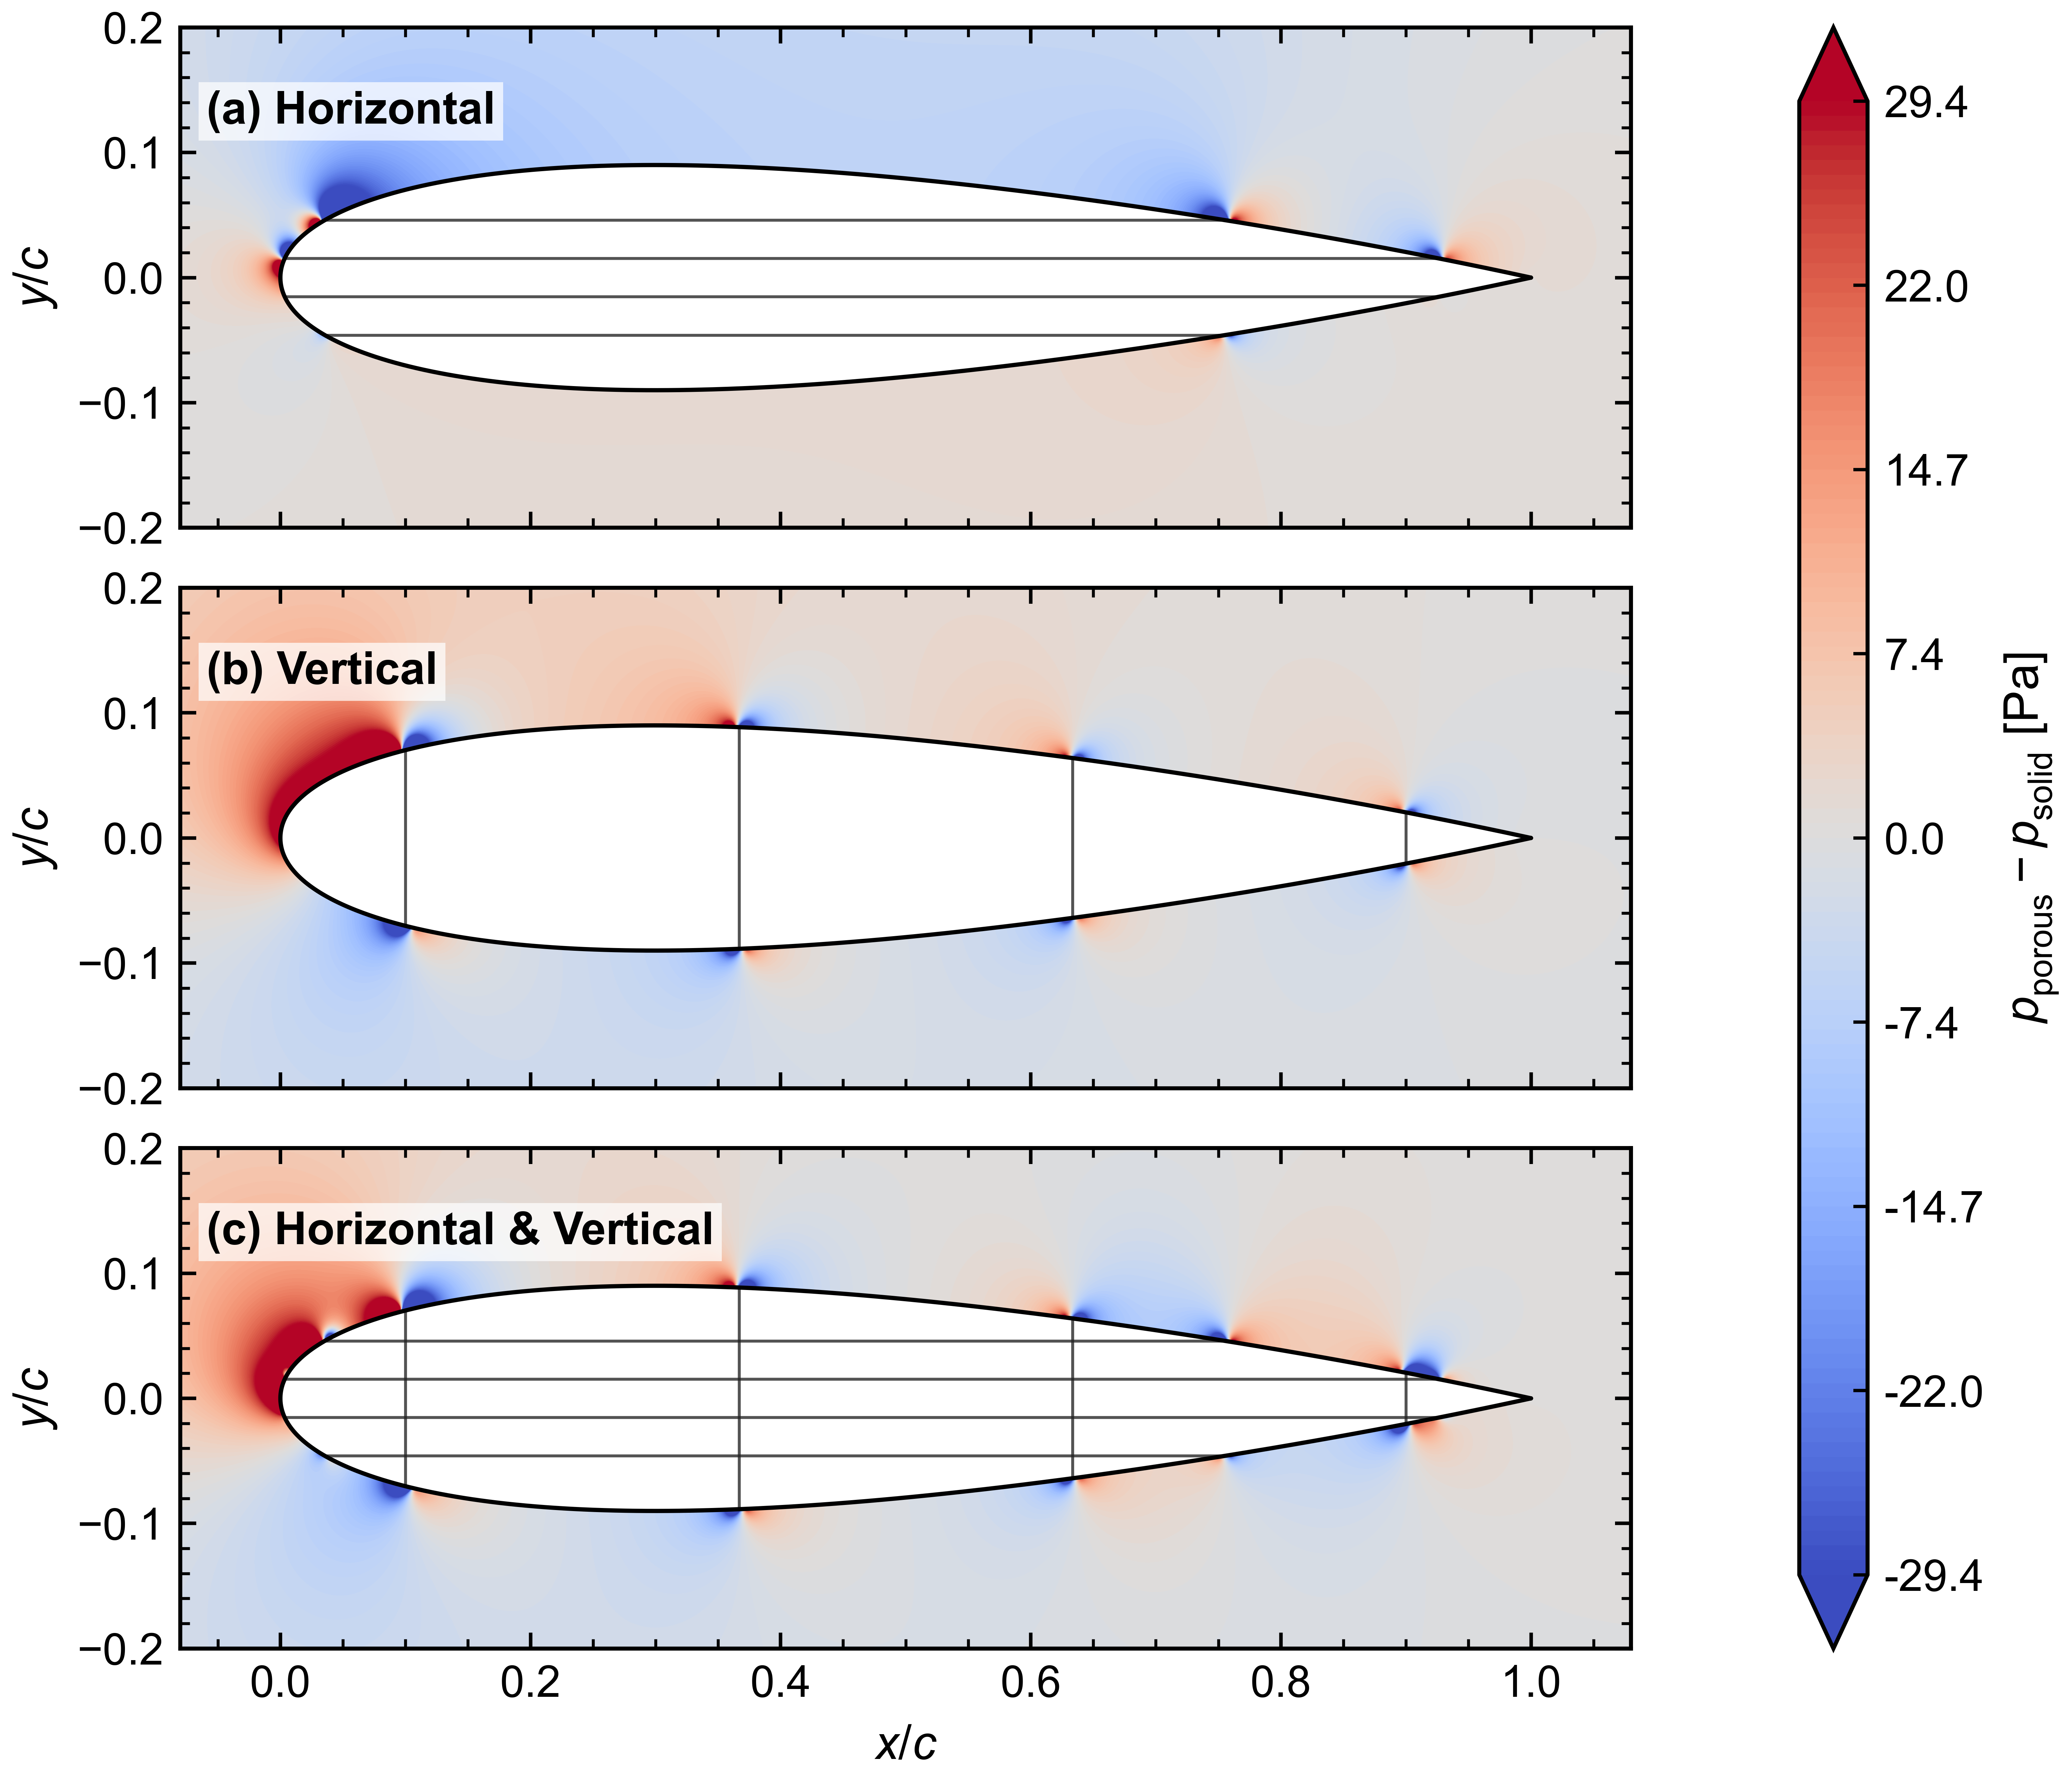
\includegraphics[
		width=0.62\textwidth
		]{figs/pressure_difference_pa_portrait_one_colorbar.png}
		\caption{{\normalfont\normalsize
				Pressure-field difference between the porous and
				impermeable airfoils at $\alpha=10^\circ$ and
				$H=9~\mathrm{mm}$ for
				(a) the horizontal porous airfoil,
				(b) the vertical porous airfoil, and
				(c) the horizontal--vertical porous airfoil.
				Positive values indicate an increase in pressure relative
				to the impermeable airfoil, while negative values indicate
				a reduction.
		}}
		\label{fig:pressure_difference}
	\end{figure*}
	
	The pressure difference is shown instead of the absolute pressure field
	to isolate the changes introduced by the pores. In the absolute
	solution, the pressure distribution is dominated by the overall
	airfoil loading and the strong pressure gradients near the leading
	edge. Subtracting the impermeable-airfoil solution makes the local
	changes associated with the pore flow easier to identify.
	
	The strongest pressure differences occur near the pore ends, where the
	internal flow directly influences the surrounding external flow. In
	several locations, neighbouring positive and negative values of
	$\Delta p$ form a dipole-like pattern. This is associated with suction
	at one end of a pore and blowing at the other, producing local regions
	of reduced and increased pressure relative to the impermeable airfoil.
	
	The effect of these pressure changes on lift depends on where they occur
	on the airfoil. At positive angle of attack, a reduction in pressure on
	the upper suction surface strengthens the suction and contributes to
	higher lift, whereas an increase in pressure has the opposite effect.
	On the lower pressure surface, an increase in pressure contributes
	positively to lift, while a pressure reduction tends to decrease it.
	
	For the horizontal porous airfoil, the pressure differences are mainly
	concentrated around the chordwise pore ends. Because both ends of each
	pore lie on the same airfoil surface, the internal flow redistributes
	pressure between different chordwise locations. The combined pressure
	changes on the upper and lower surfaces increase the pressure difference
	across the airfoil, consistent with the higher lift coefficient observed
	for this configuration.
	
	The vertical porous airfoil produces a different pattern because each
	pore connects the pressure surface to the suction surface. Flow is
	therefore driven from the higher-pressure region towards the
	lower-pressure region, producing local pressure changes at both pore
	ends. At the same time, this cross-surface flow partially reduces the
	pressure difference between the two surfaces, which is consistent with
	the lower lift coefficient obtained for the vertical configuration.
	
	The horizontal--vertical porous airfoil contains features associated
	with both pore arrangements. The horizontal pores redistribute pressure
	along the airfoil surfaces, while the vertical pores transfer flow
	between the pressure and suction surfaces. Although the two pore systems
	remain physically separate and hydraulically independent, their
	aerodynamic effects interact through the external pressure field.
	Consequently, the pressure equalisation associated with the vertical
	pores partly counteracts the pressure redistribution produced by the
	horizontal pores, giving an overall aerodynamic behaviour closer to
	that of the impermeable airfoil.
	
	% ============================================================
	% VELOCITY FIELD
	% ============================================================
	
	\subsubsection{Velocity field characteristics}
	
	\begin{figure*}
		\centering
		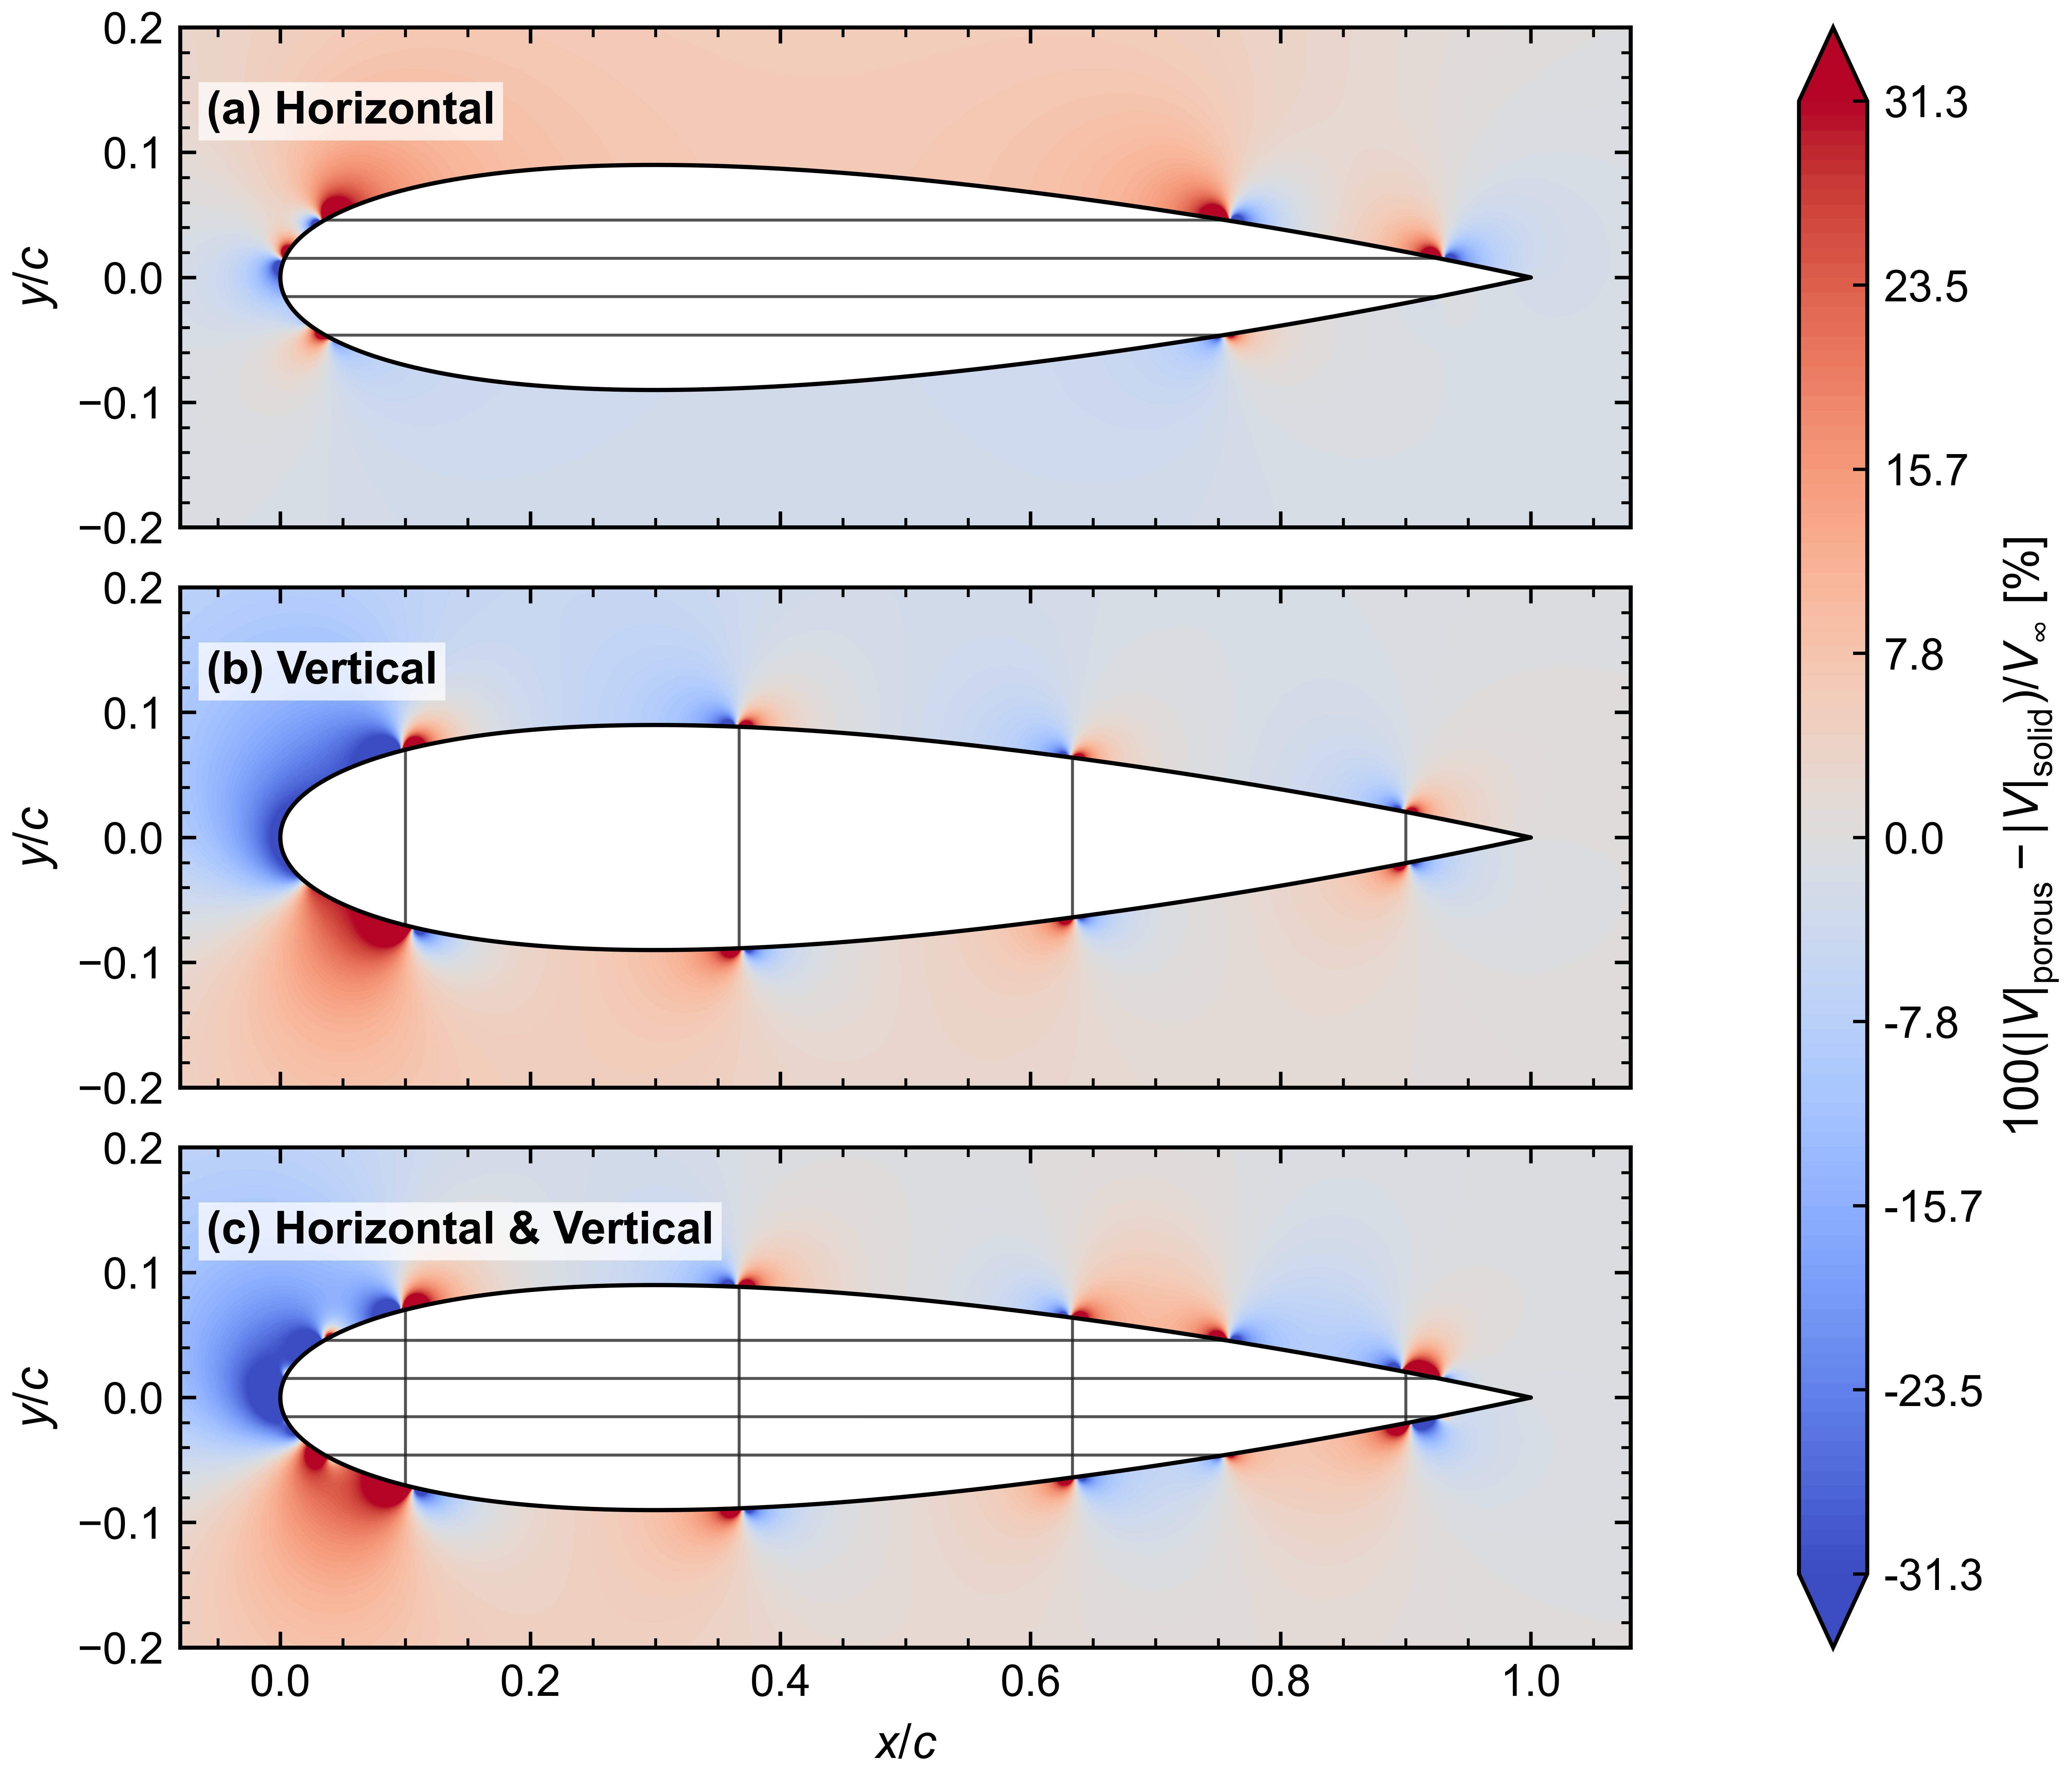
\includegraphics[
		width=0.62\textwidth
		]{figs/velocity_difference_percent_portrait_one_colorbar.png}
		\caption{{\normalfont\normalsize
				Percentage difference in velocity magnitude between the porous
				and impermeable airfoils at $\alpha=10^\circ$ and
				$H=9~\mathrm{mm}$ for
				(a) the horizontal porous airfoil,
				(b) the vertical porous airfoil, and
				(c) the horizontal--vertical porous airfoil.
				Positive values indicate an increase in velocity magnitude,
				while negative values indicate a reduction relative to the
				impermeable airfoil.
		}}
		\label{fig:velocity_difference}
	\end{figure*}
	
	The velocity field is presented as the percentage difference relative
	to the impermeable-airfoil solution,
	
	\begin{equation}
		\Delta |\boldsymbol{V}|_{\%}
		=
		\frac{
			|\boldsymbol{V}|_{\mathrm{porous}}
			-
			|\boldsymbol{V}|_{\mathrm{solid}}
		}{
			|\boldsymbol{V}|_{\mathrm{solid}}
		}
		\times 100.
		\label{eq:velocity_field_difference}
	\end{equation}
	
	This comparison isolates the changes introduced by the pores from the dominant background flow around the airfoil. The largest velocity differences occur close to the pore ends,
	where the imposed surface-normal flow locally perturbs the external
	velocity field. Adjacent regions of acceleration and deceleration are
	visible around several pores and correspond closely to the pressure
	patterns shown in Figure.~\ref{fig:pressure_difference}.
	
	The velocity and pressure fields show the expected inverse relationship
	described by Bernoulli's equation. Regions where the flow accelerates
	are generally associated with a reduction in static pressure, whereas
	regions of lower velocity correspond to higher static pressure. The
	velocity contours therefore help explain how the pore-induced changes
	in the local flow field lead to the observed pressure redistribution
	and, consequently, changes in the aerodynamic forces and pitching
	moment.
	
	For the horizontal porous airfoil, alternating regions of acceleration
	and deceleration are concentrated around the chordwise pore ends. Since
	both ends of each pore lie on the same airfoil surface, the internal
	flow redistributes the external velocity between different chordwise
	locations. The combined changes on the suction and pressure surfaces
	strengthen the pressure difference across the airfoil, consistent with
	the increase in lift and the larger change in pitching moment observed
	for this configuration.
	
	The vertical porous airfoil shows a different velocity pattern. Flow
	between the pressure and suction surfaces changes the external velocity
	on both sides of the airfoil and reduces part of the velocity contrast
	between them. This behaviour is consistent with the partial pressure
	equalisation discussed previously and the corresponding reduction in
	lift. A broader region of velocity difference is also visible near the
	leading edge, where the external flow experiences strong pressure and
	velocity gradients.
	
	The horizontal--vertical porous airfoil contains features associated
	with both pore arrangements. The horizontal pores produce local
	chordwise acceleration and deceleration, while the vertical pores
	redistribute flow between the pressure and suction surfaces. Although
	the two pore arrangements remain physically separate and hydraulically
	independent, their aerodynamic effects interact through the external
	flow field. The resulting velocity distribution therefore reflects the
	combined influence of both mechanisms rather than a simple
	superposition of the individual configurations.
	
	Overall, the velocity contours support the trends observed in the
	pressure field and aerodynamic coefficients. The horizontal pores
	primarily redistribute the flow along the airfoil surfaces, whereas the
	vertical pores transfer flow between the pressure and suction surfaces.
	These different flow mechanisms contribute to the contrasting lift and
	pitching-moment behaviour of the three porous-airfoil configurations.
	

	
	\section{Conclusion}
	
	\bibliographystyle{elsarticle-num}
	\bibliography{porous_airfoil_literature_COMPLETE}
\end{document}

}